\documentclass[12pt,draft]{mitthesis} 

\usepackage{lgrind, braket, amsmath,
  amssymb, bbm, booktabs, subfig, color} 

\usepackage[pdftex]{graphicx}
\usepackage[version=3]{mhchem}

\newcommand{\TODO} [1]{\textcolor{magenta}{\textbf{TODO:} #1}}
\newcommand{\NOTE} [1]{\textcolor{magenta}{[\emph{#1}]}}
\newcommand{\POINT}[1]{\textcolor{magenta}{#1}}

\newcommand{\rcm}{cm$^{-1}$}
\newcommand{\bigspace}{$
  \;
  $}

\newcommand{\astate}{$
  \tilde{\text{A}} \: ^1\!A_u
  $}
\newcommand{\AtoX}{$
  \tilde{\text{A}} \: ^1\!A_u 
  \leftarrow 
  \tilde{\text{X}} \: ^1\Sigma_g^+
  $}
\newcommand{\StoS}{$
  S_1 \leftarrow S_0
  $}
\newcommand{\microsec}{$\mu$s}

\hyphenation{acetylene}
\hyphenation{Hamiltonian}

\begin{document}

\tableofcontents
\clearpage

\subsubsection*{NOTES}

\clearpage

\setcounter{chapter}{3}
\chapter{SEELEM/LIF spectroscopy of acetylene: 
Spectral patterns of mediated spin-orbit coupling
in a near iso-energetic set of vibrational levels
}

\section{Introduction}

The dynamics of singlet$\sim$triplet coupling in the \AtoX \bigspace
(\StoS) electronic spectrum of acetylene, \ce{C2H2}, have been
extensively studied.  This body of work establishes a heirarchical
model for electronic coupling, which leads to the effects of
intersystem crossing and internal conversion: $S_1 \rightarrow T_3
\rightarrow T_{1,2} \rightarrow S_0$.  Top-tier interactions between
the $S_1$ and $T_3$ electronic states are of particular interest
because (1) they control coupling to the remaining electronic states
of the molecule and (2) they are primarily determined by vibrational
overlap factors and energy denominators, two sensitive consequents of
the molecule's electronic structure.

Surface Electron Ejection by Laser-Excited Metastables \cite{sneh89,
  sneh91, humphrey97} (SEELEM) and LIF spectroscopy are complementary
techniques, which, when used together, can provide information about
$S_1 \sim T_3$ interactions \cite{humphrey97, mishra04, altunata00,
  altunata02}.  \TODO{Finish adapting from paper.}  LIF detection is
limited to short-lived ($\tau_{radiative}<$ 10 \microsec), strongly
fluorescing states, while SEELEM detection is sensitive only to
long-lived ($\tau >$ 300 \microsec) states with vertical electronic
excitation above a threshold energy set by the work function of the
metal used as the SEELEM detector surface. Therefore, SEELEM and LIF
detection channels observe mutually exclusive sets of eigenstates that
arise from spin-orbit mixed $S_1$ and $T_{3,2,1}$ zero-order basis
states.  Because SEELEM detection is sensitive to the electronic
character of the molecule, a comparison of simultaneously recorded
SEELEM and LIF spectra reveals features of electronic structure and
photochemical pathways that are invisible via traditional,
single-channel spectroscopic probes such as LIF alone, REMPI,
phosphorescence, or phosphor surface \cite{shi98, campos01, burton72}.
% Information gained from comparison of acetylene SEELEM
% and LIF spectra can yield a mechanistic description of
% singlet$\sim$triplet interaction, and holds promise for describing the
% structure and dynamics of other small polyatomic species \cite{jung07,
%   allen07}.
% SEELEM spectroscopy has
% been used in this effort as a tool to examine $S_1 \sim T_3$ coupling,
% by allowing detection of the local manifold of predominantly $T_{1,2}$
% eigenstates in the region surrounding an \StoS\ transition.

The \emph{trans}-bending mode of $S_1$ acetylene, $\nu_3$, is known to
be an important promoter of singlet$\sim$triplet coupling.  In Zeeman
anticrossing experiments, Dupr\'{e} and coworkers observed a rapid
increase in the anticrossing density, as well as the product
$\rho_{\text{vib}} \braket{H_{st}}$, with energy in $\nu_3$
\cite{dupre91, dupre95b}.  They also observed an single large
singlet$\sim$triplet anticrossing in the $3 \nu_3$ $K_a=0$ level,
%with a zero-field matrix element of 0.29 \rcm,
which was in turn perturbed by many smaller couplings \cite{dupre93}.
These observations led the authors to propose that the
singlet$\sim$triplet dynamics of acetylene in the \astate\ state are
best described by a doorway-mediated mechanism, in which particular
triplet vibrational levels mediate intersystem crossing between the
initially excited $S_1$ bright state and the dense manifold of highly
mixed, dark $T_{1,2}$ states.  Subsequent theoretical and experimental
work confirmed that the coupling doorways were vibrational levels of
the $T_3$ electronic state \cite{vacek96, sherrill96, humphrey97,
  altunata00}.

The $S_1$ $3 \nu_3$ $K_a$=1 level has been heavily studied due to a
local $S_1 \sim T_3$ level crossing at $J \approx 3$.  Spectroscopic
patterns in SEELEM arising from the effects of the local $T_3$
perturber in have been discussed by several authors \cite{humphrey97,
  altunata00, altunata01, mishra04}.  Using vibrational overlap
integrals gained from \emph{ab initio} calculations of the $T_3$
electronic surface, Thom and coauthors were able to exclude all but
several candidate $T_3$ levels as the local triplet perturber in $S_1$
$3 \nu_3$ $K_a$=1 \cite{thom07}.
% \POINT{Overlap between $S_1$ and $T_3$ levels predicted by Bryan and
%   Ryan.  (See p.40 of 1/2007--3/2007 notebook.)}
However, recent observations of an increase in $S_1 \sim T_{1,2}$
coupling at higher values of $J$ suggest that the local $T_3$
perturber is not the sole, and perhaps not the primary, doorway for
$3 \nu_3$ \cite{degroot07}.

That an energetically distant doorway, which would be required to have
a correspondingly larger spin-orbit matrix element, may play a role in
coupling $S_1$ $3 \nu_3$ to the $T_{1,2}$ manifold is not altogether
surprising, given the energy region in question.  \emph{Ab initio}
calculations are in agreement that an electronic surface crossing
between the $S_1$ and $T_3$ states is energetically nearby
\cite{ventura03, thom07}.  Such a surface crossing would allow for
strong interactions with several $T_3$ levels in the same energy
region.  It should also play a role in promoting singlet$\sim$triplet
coupling within other $S_1$ levels in the same energy region.  The
$4\nu_3$ level, 1000 \rcm\ higher in energy, is also strongly coupled
to the $T_{1,2}$ manifold, although no obvious local $T_3$ doorway has
been observed \cite{drabbels93, ochi91}.

The energies of the $3 \nu_3$ and $4\nu_3$ levels can therefore be
taken as conservative lower and upper bounds for such an $S_1 \sim
T_3$ ``active'' coupling region.  We turn our attention to other
vibrational levels of $S_1$, which, while in this critical energy
region, are not near-degenerate with a mediating $T_3$ level at low
$J$.  The levels chosen for study all lie within 500 \rcm\ of $3
\nu_3$ $K_a$=1, and involve excitation in only the Franck-Condon
active modes of $S_1$ acetlyene, $\nu_2$ (C-C stretch) and $\nu_3$
(\emph{trans} bend).

The coupling between these $S_1$ levels and the local manifold of
$T_{1,2}$ states is expected, in this case, to be mediated by
energetically distant $T_3$ levels.  Evidence for energetically
distant, mediating $T_3$ levels is obtained by comparing
simultaneously recorded LIF and SEELEM spectra, and a new technique
for comparison is developed to suit this purpose.  This new technique
takes into account shifting intensity patterns in the frequency-domain
LIF spectrum as a function of delay time, due to the time development
of an incoherent ensemble of eigenstates with different fluorescence
lifetimes.  When used on a segment of spectrum that includes just one
singlet rovibronic transition, the technique reveals a
coupling-dependent shift in the statistical properties of the
spectrum.  Comparison with other transitions in a rotational series
can reveal local perturbations caused by weakly coupled $T_3$ levels.
When used on a spectrum containing several rovibronic transitions in
series, the technique can give insight into the matrix element and
relative energy of a $T_3$ doorway level.

\section{Patterns of spectral intensity in gated fluorescence and
  SEELEM}

In Chapter 2, we introduced the concept of a SEELEM intensity
distribution associated with a singlet bright state.  Here, we extend
the idea of dark state intensity distributions to fluorescence
measurements by considering intensities in the \emph{incoherent,
  frequency domain} LIF spectrum at a time window $t+dt$ after
excitation of the molecule.  The SEELEM spectrum is shown to be an
extreme, limiting case of delayed fluorescence.  Furthermore, we
demonstrate that molecular properties such as coupling matrix element
and the energy denominator for a mediating doorway state are revealed
by changes in statistical properties of the spectrum as it changes
from sub-\microsec\ gated LIF, into delayed LIF, and finally to
SEELEM.

\TODO{Adapt following from delayedfluorescence report.}  For a pure
singlet bright state $\ket{s}$, the time-dependent fluorescence
intensity is
\begin{equation}
  I_s(t) = \frac{1}{\tau_s} \;
           \exp \left[
             -\frac{t}{ \tau_s} 
           \right],
\end{equation}
normalized such that $\int_0^{\infty} I_s(t) \, dt = 1$.

We consider the case where $\ket{s}$ is directly coupled with a set of
$N$ triplet dark states to create a set of $N$+1 mixed states
$\lbrace\ket{m}\rbrace$.  Each state $\ket{m}$ has some bright state
amplitude $a_m$.  In the case of direct or doorway-mediated coupling,
the Hamiltonian contains only one pathway from each dark state to the
bright state (see Chapter 3).  As a result, the mixing amlitudes may
be taken to be real and positive by convention.  If the lifetime of a
pure triplet dark state is much longer than $\tau_s$, the lifetime of
a mixed eigenstate $\ket{m}$ having bright state character
$\alpha_m^2$ is
\begin{equation}
  \label{eq:tau-m}
  \tau_m = \tau_s / a_m^2,
\end{equation}
and its time-dependent fluorescence intensity is
\begin{equation}
  \label{eq:int-m}
  I_m(t) = \frac{a_m^4}{\tau_s} \;
           \exp \left[
             -\frac{a_m^2 \, t}{\tau_s} 
           \right].
\end{equation}
The total integrated fluorescence intensity for a mixed state is
$\int_0^{\infty} I_m(t) \, dt = a_m^2$, relative to unit intensity for
a pure bright state.

The normalization condition for bright state character $\sum_m a_m^2 =
1$ leads to the relation
\begin{equation}
  \tau_s^{-1} = \sum_m \tau_m^{-1};
\end{equation}
in this way, $\tau_s$ can be derived from the set of mixed state
lifetimes $\lbrace \tau_m \rbrace$.

\subsection{SEELEM detection as an extreme limit of delayed fluorescence}

We examine the fluorescence intensity after a time delay $t_c$,
which we cast in units of the bright state lifetime:
\begin{equation}
  R_c = t_c / \tau_s.
\end{equation}
At a chosen $R_c$, the fluorescence intensity equation has a single
peak according to some value of bright state character.  Within the
range $0 \le a_m^2 \le 1$, the fluorescence intensity equation is at a
maximum when (Chapter 2, equation 31)
\begin{equation}
  \label{eq:am-max}
  a_m^2 = \frac{2}{R_c}.
\end{equation}

\begin{figure}
  \caption{The intensity of a mixed eigenstate at time $R_c =
    t/\tau_s$, plotted as a function of bright
    state character.}
  \label{fig:int-at-rc}
  \centering
  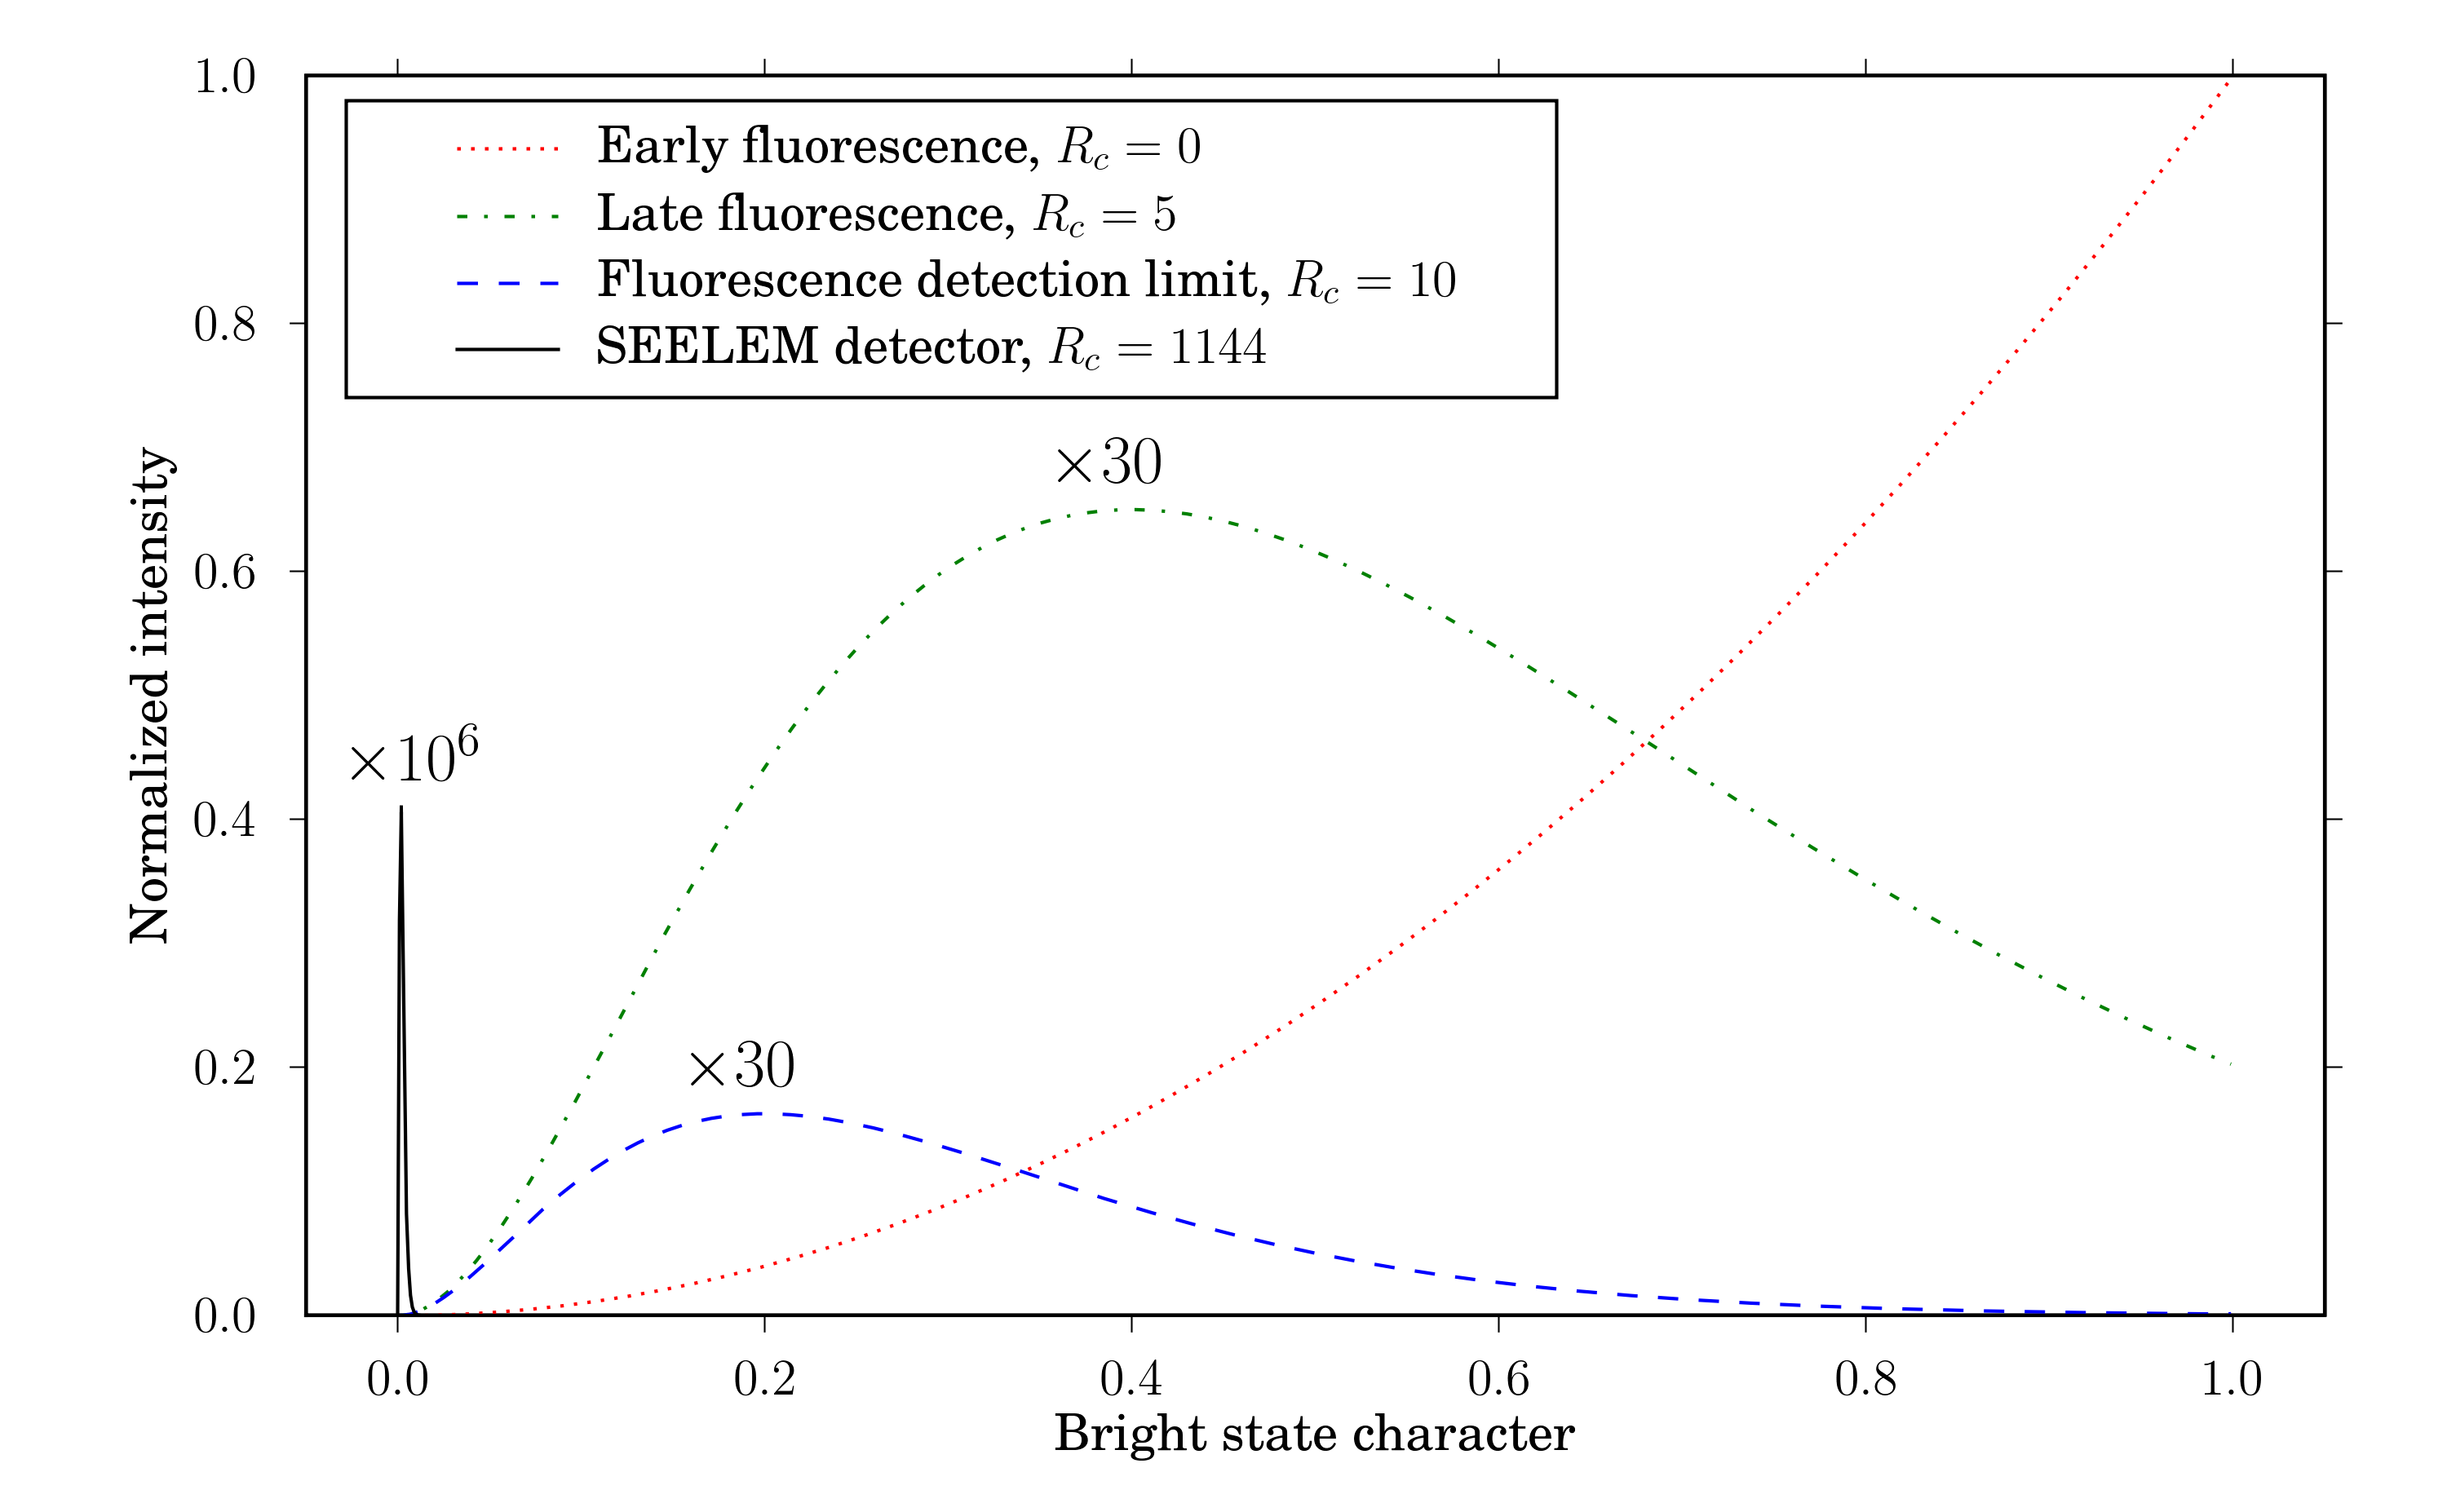
\includegraphics[width=7.5in,angle=90]{intensity-at-rc.png}
\end{figure}

Figure \ref{fig:int-at-rc} shows the dependence of fluorescence
intensity on bright state character for several values of $R_c$.  At
early fluorescence times ($\sim \tau_s$), the fluorescence intensity
is greatest for states with large amounts of bright state character
($2/R_c > 1$).  At a delay of $5 \tau_s$, the fluorescence intensity
equation discriminates against states with large amounts of bright
state character, since molecules in such states have already
fluoresced with high probability.  States with small amounts of bright
state character are also discriminated against -- molecules in these
states have a low probability of fluorescing at the time under
consideration.  The fluorescence intensity is thus ``tuned'' to a
particular value of bright state character at every time delay $R_c$,
according to Equation \ref{eq:am-max}.

Note that the intensity expression used here does not account for
molecules leaving the field of view of the fluorescence detection
optics.  We consider only the distribution of bright state character
\emph{among molecules remaining in the field of view at time $R_c$}.
However, since there is no momentum transfer from the excitation
photon to the molecule, the rate of molecules exiting the field of
view is independent of bright state character.  Therefore,
simple reasoning according to the above intensity formulas will be
correct as long as we discuss fluorescence intensities only in terms
of ratios.

To foster a more concrete discussion, consider our experiments on
intersystem crossing in acetylene.  For the $S_1$ electronic state,
$\tau_s=270$ ns.  In our apparatus, the field-of-view of the
fluorescence detection optics is several mm, which amounts to a
maximum viewing time of 3 $\mu$s, about $10\tau_s$, for molecules in
the molecular beam with a velocity of $10^3$ m/s.  At times later than
$10\tau_s$, there are simply no molecules left to observe in the
fluorescence field of view.  This places an upper limit on the value
of $R_c$ that can be examined in our fluorescence experiments.  Figure
\ref{fig:int-at-rc} shows the intensity equation for the limit of
fluorescence detection, $10\tau_s$.

The SEELEM detector used in our experiments detects metastable
molecules after a 309 $\mu$s flight time.  If we set aside some
particularly interesting aspects of SEELEM detectivity and consider
only its detection sensitivity to bright state character, we arrive at
the following equation for SEELEM detection probability (Chapter 2,
equation 28):
\begin{equation}
  \label{eq:seelem-prob-s}
  P_{SEELEM}^{(s)} \propto a_m^4 \; \exp \left( -R_c \, a_m^2 \right).
\end{equation}
(This is a good approximation to its overall detection sensitivity,
including $T_3$, in the weak coupling limit.)  The SEELEM detection
probability equation above has the same functional form as the
Equation \ref{eq:int-m}.  Thus, the SEELEM detector may be viewed in
this limited sense as an extreme discriminator for states with small
amounts of bright state character.

Acetylene molecules in our apparatus are detected after an average
flight time of 309 $\mu$s, yielding an $R_c$ value of $1144$ for the
SEELEM detector.  This corresponds to a maximum detection probability
for states with $0.17\%$ bright state character.

\subsection{Delayed fluorescence of a two-level system}

Our next step is to examine the changing characteristics of a
fluorescence intensity distribution as we increase the time delay
$R_c$.  We model the interaction between a bright state and an
ensemble of dark states by generalizing from a two-level system.
Consider a Hamiltonian with only one dark state.  Define the two mixed
states $\ket{m=1,2}$ as
\begin{equation}
  \begin{split}
    \ket{1} &=  (1 - \alpha^2)^{1/2} \ket{s} + \alpha \ket{t}\\
    \ket{2} &= -\alpha \ket{s} + (1 - \alpha^2)^{1/2} \ket{t}.
  \end{split}
\end{equation}
The fluorescence intensity of both states, relative to a pure bright
state, is
\begin{equation}
  \begin{split}
    I_1 &= \frac{(1 - \alpha^2)^2}{\tau_s} \; \exp 
          \left[
            - R_c \, (1 - \alpha^2)
          \right]\\
    I_2 &= \frac{\alpha^4}{\tau_s} \; \exp 
          \left[
            - R_c \, \alpha^2
          \right],
  \end{split}
\end{equation}
and the ratio of the fluorescence intensities changes with time as
\begin{equation}
  I_{12} = I_1 / I_2 = 
  \left(
    \frac{(1 - \alpha^2)}{\alpha^2}
  \right)^2
  \exp
  \left[
    - R_c \, (1 - 2\alpha^2)
  \right].
\end{equation}
The fluorescence intensity ratio may be used to write an equation for
the dependence of average intensity on $R_c$.
\begin{equation}
  \label{eq:ratio}
  \braket{I_{LIF}} = 
  \frac{\Delta E_{12}}{2} \,
  \left(
    \frac{I_{12}-1}{I_{12}+1}
  \right)
\end{equation}
Figure \ref{fig:ratio} shows the dependence of center-of-gravity on
the intensity ratio $I_{12}$.

\begin{figure}
  \caption{Center of gravity as a function of the intensity ratio
    $I_1$:$I_2$ for a two-state system.  At $t=0$, the initial center
    of gravity is a function of the mixing amplitude $\alpha$.  The
    center of gravity then shifts with the changing intensity ratio as
    delay time is increased, arriving at a limiting value of $-\Delta
    E_{12}/2$.}
  \label{fig:ratio}
  \centering
  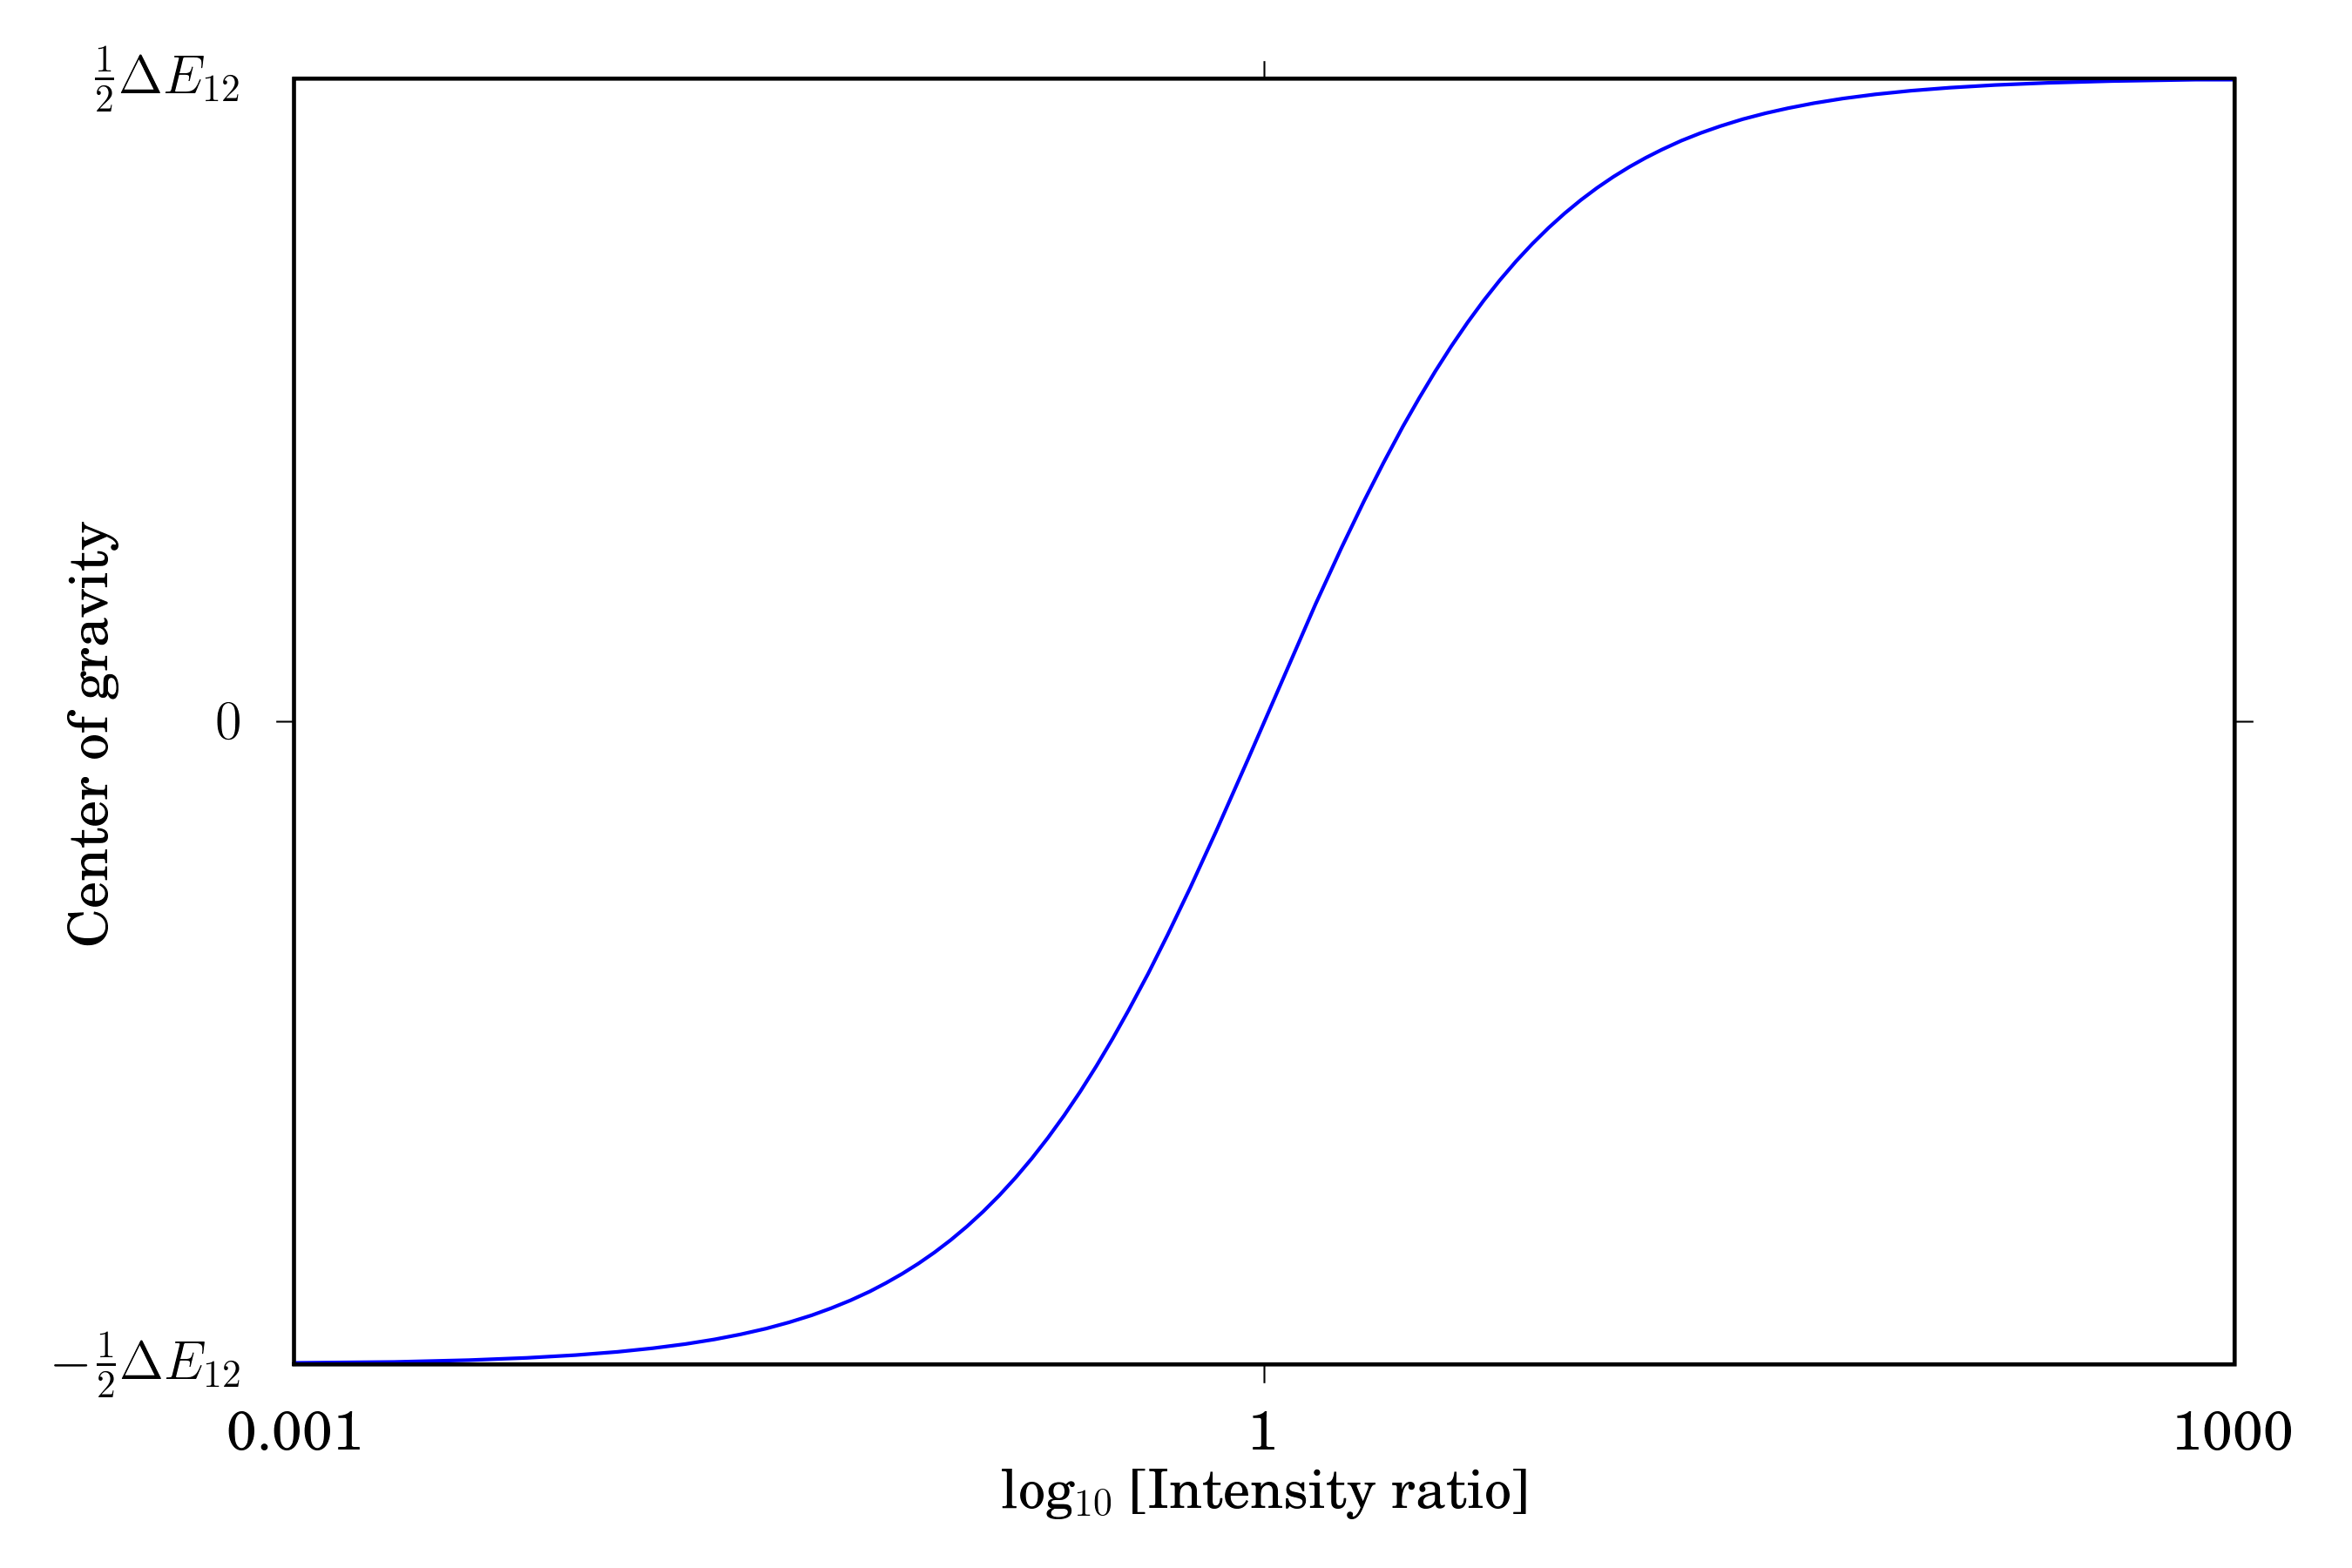
\includegraphics[width=6in]{cog-from-ratio.png}
\end{figure}

The initial intensity ratio at time $R_c=0$ is
\begin{equation}
  I_{12} = 
  \left(
    \frac{(1 - \alpha^2)}{\alpha^2}
  \right)^2.
\end{equation}
From this, the initial center of gravity can be found according to
Equation \ref{eq:ratio} or Figure \ref{fig:ratio}.  At large values of
$R_c$, the intensity ratio decreases to zero as $I_1 \ll I_2$, if the
states are not 50:50 mixed.  As the ratio decreases to zero, the
center of gravity approaches $-\Delta E_{12} / 2$.  The development of
intensity ratios and the consequent shift in center of gravity are
shown in Figure \ref{fig:cog-devel}.  One interesting aspect of the
center of gravity shift shown in the figure is the rapid onset of the
shift at small mixing coefficients.

\begin{figure}
  \caption{(Top) Time development of the relative intensity ratio for
    a two state system. (Bottom) Time development of the center of
    gravity for a two state system.}
  \label{fig:cog-devel}
  \centering
  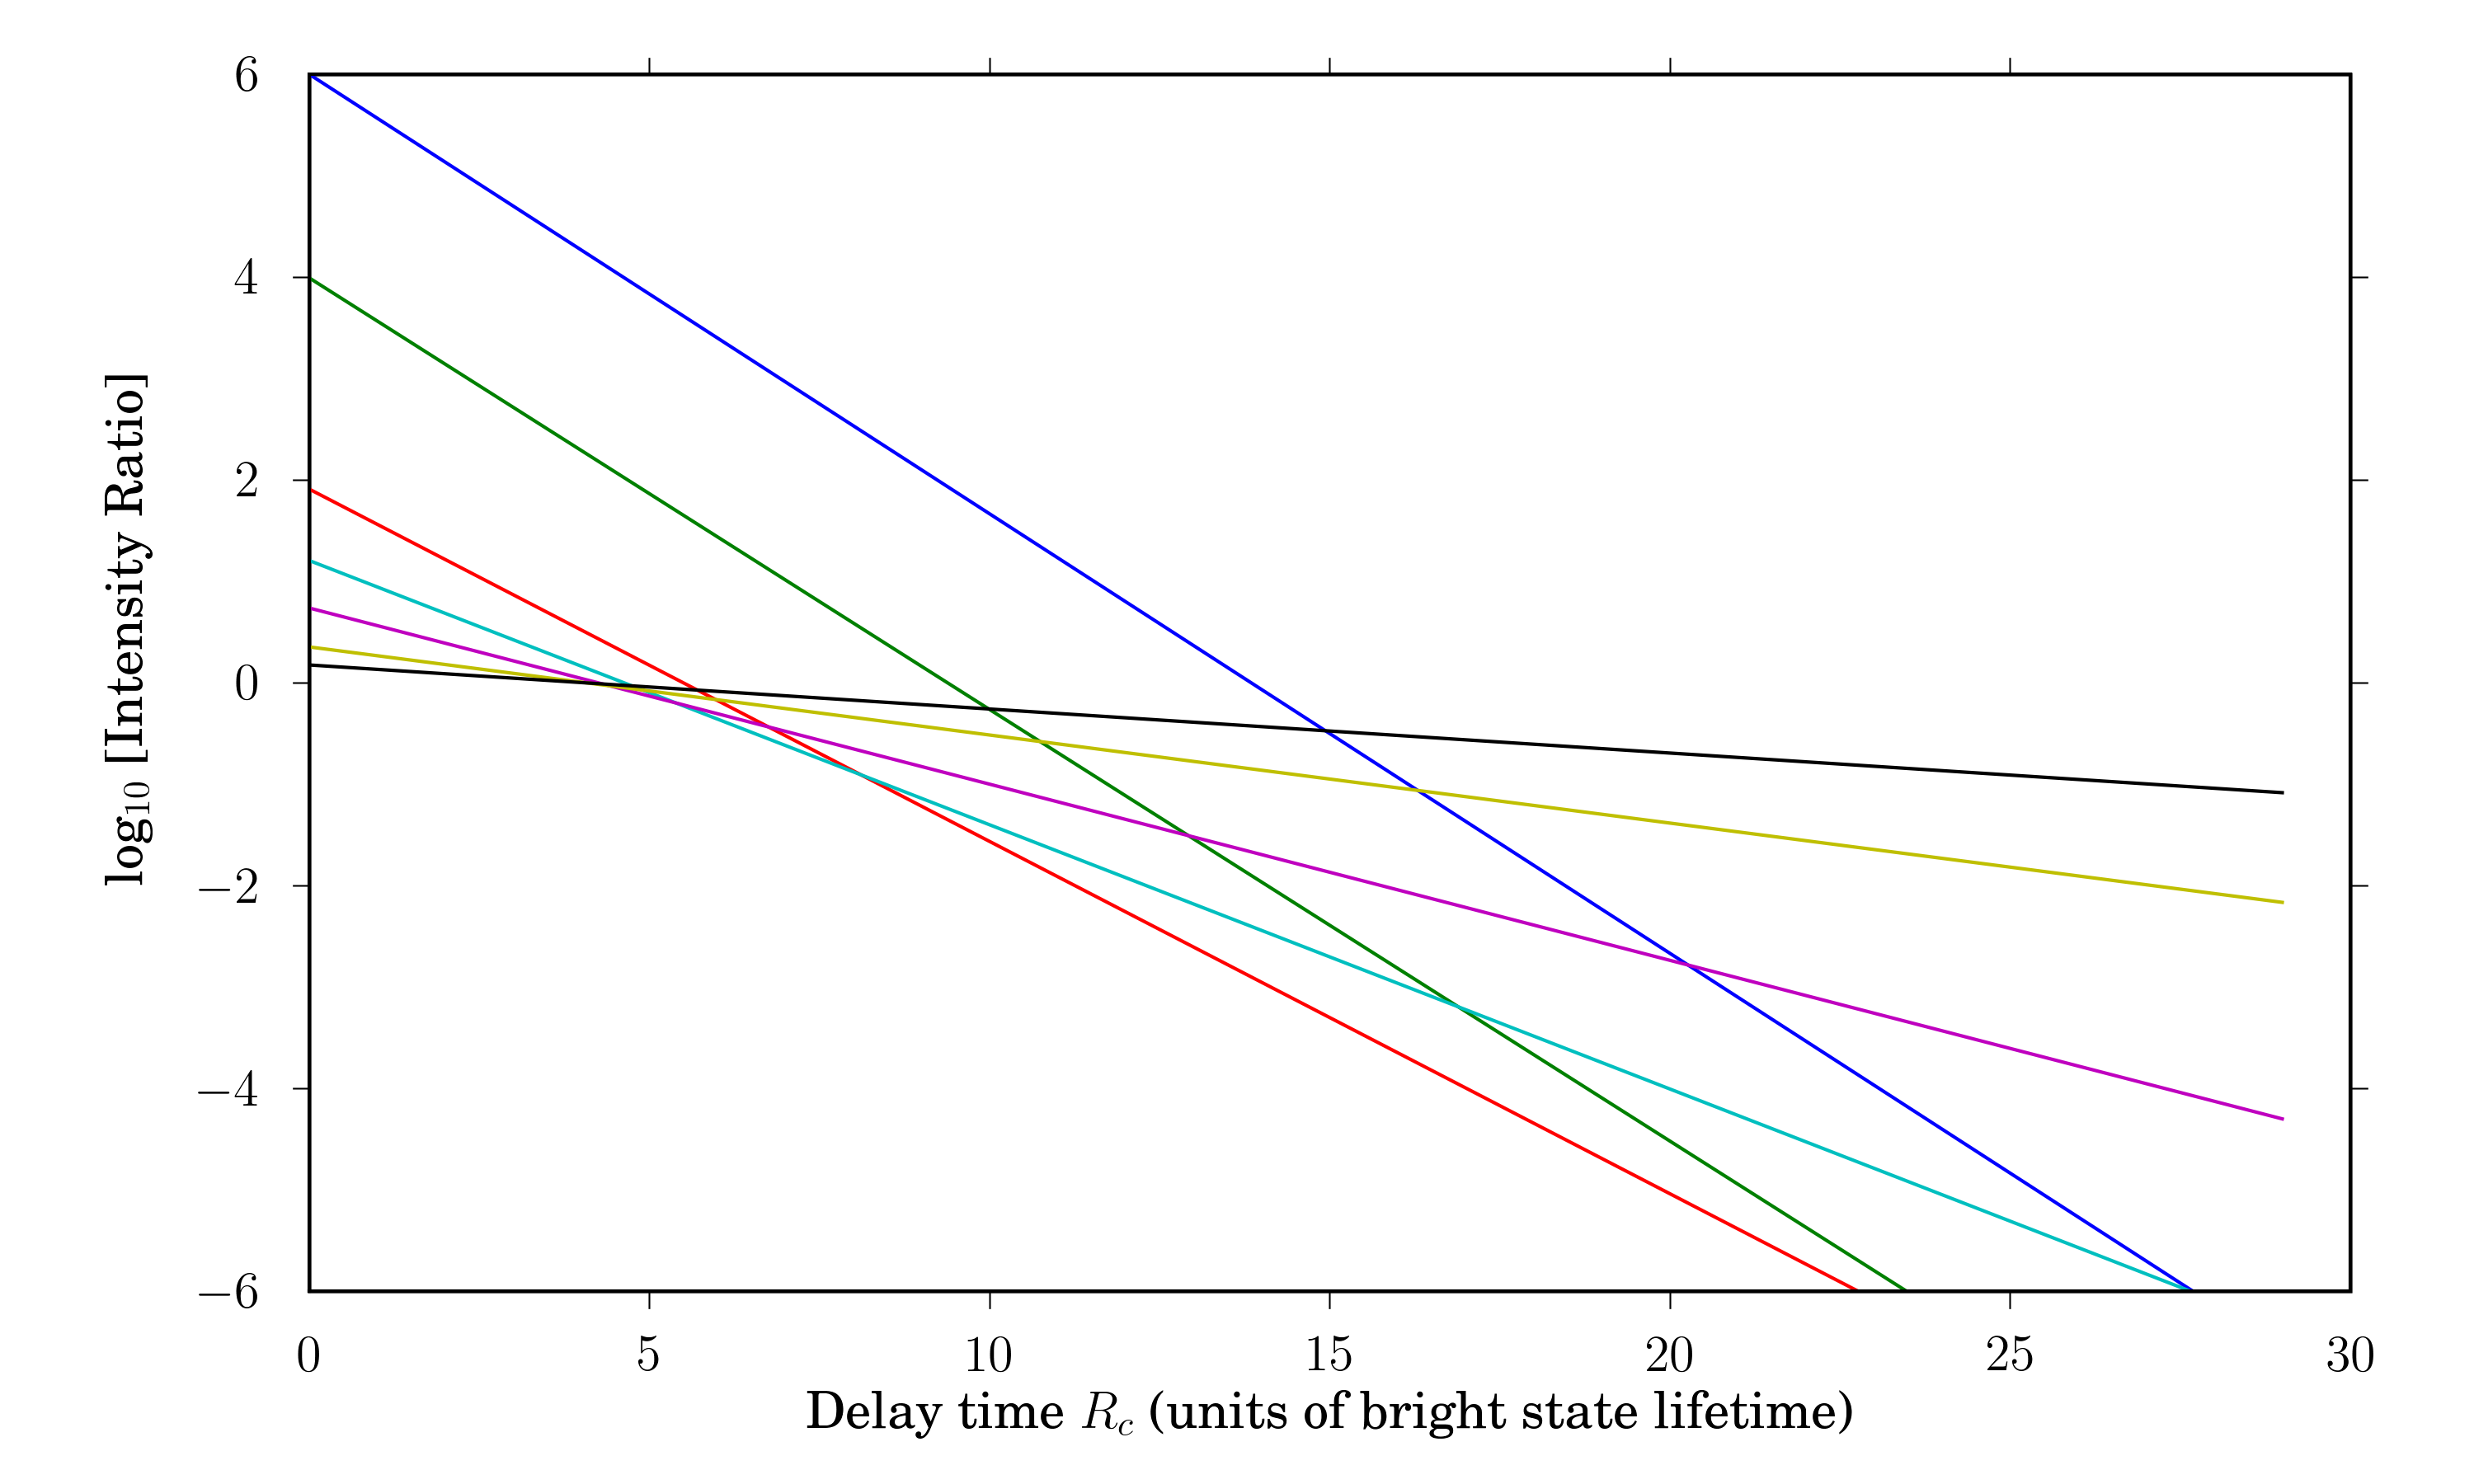
\includegraphics[width=6in]{ratio-development.png}
  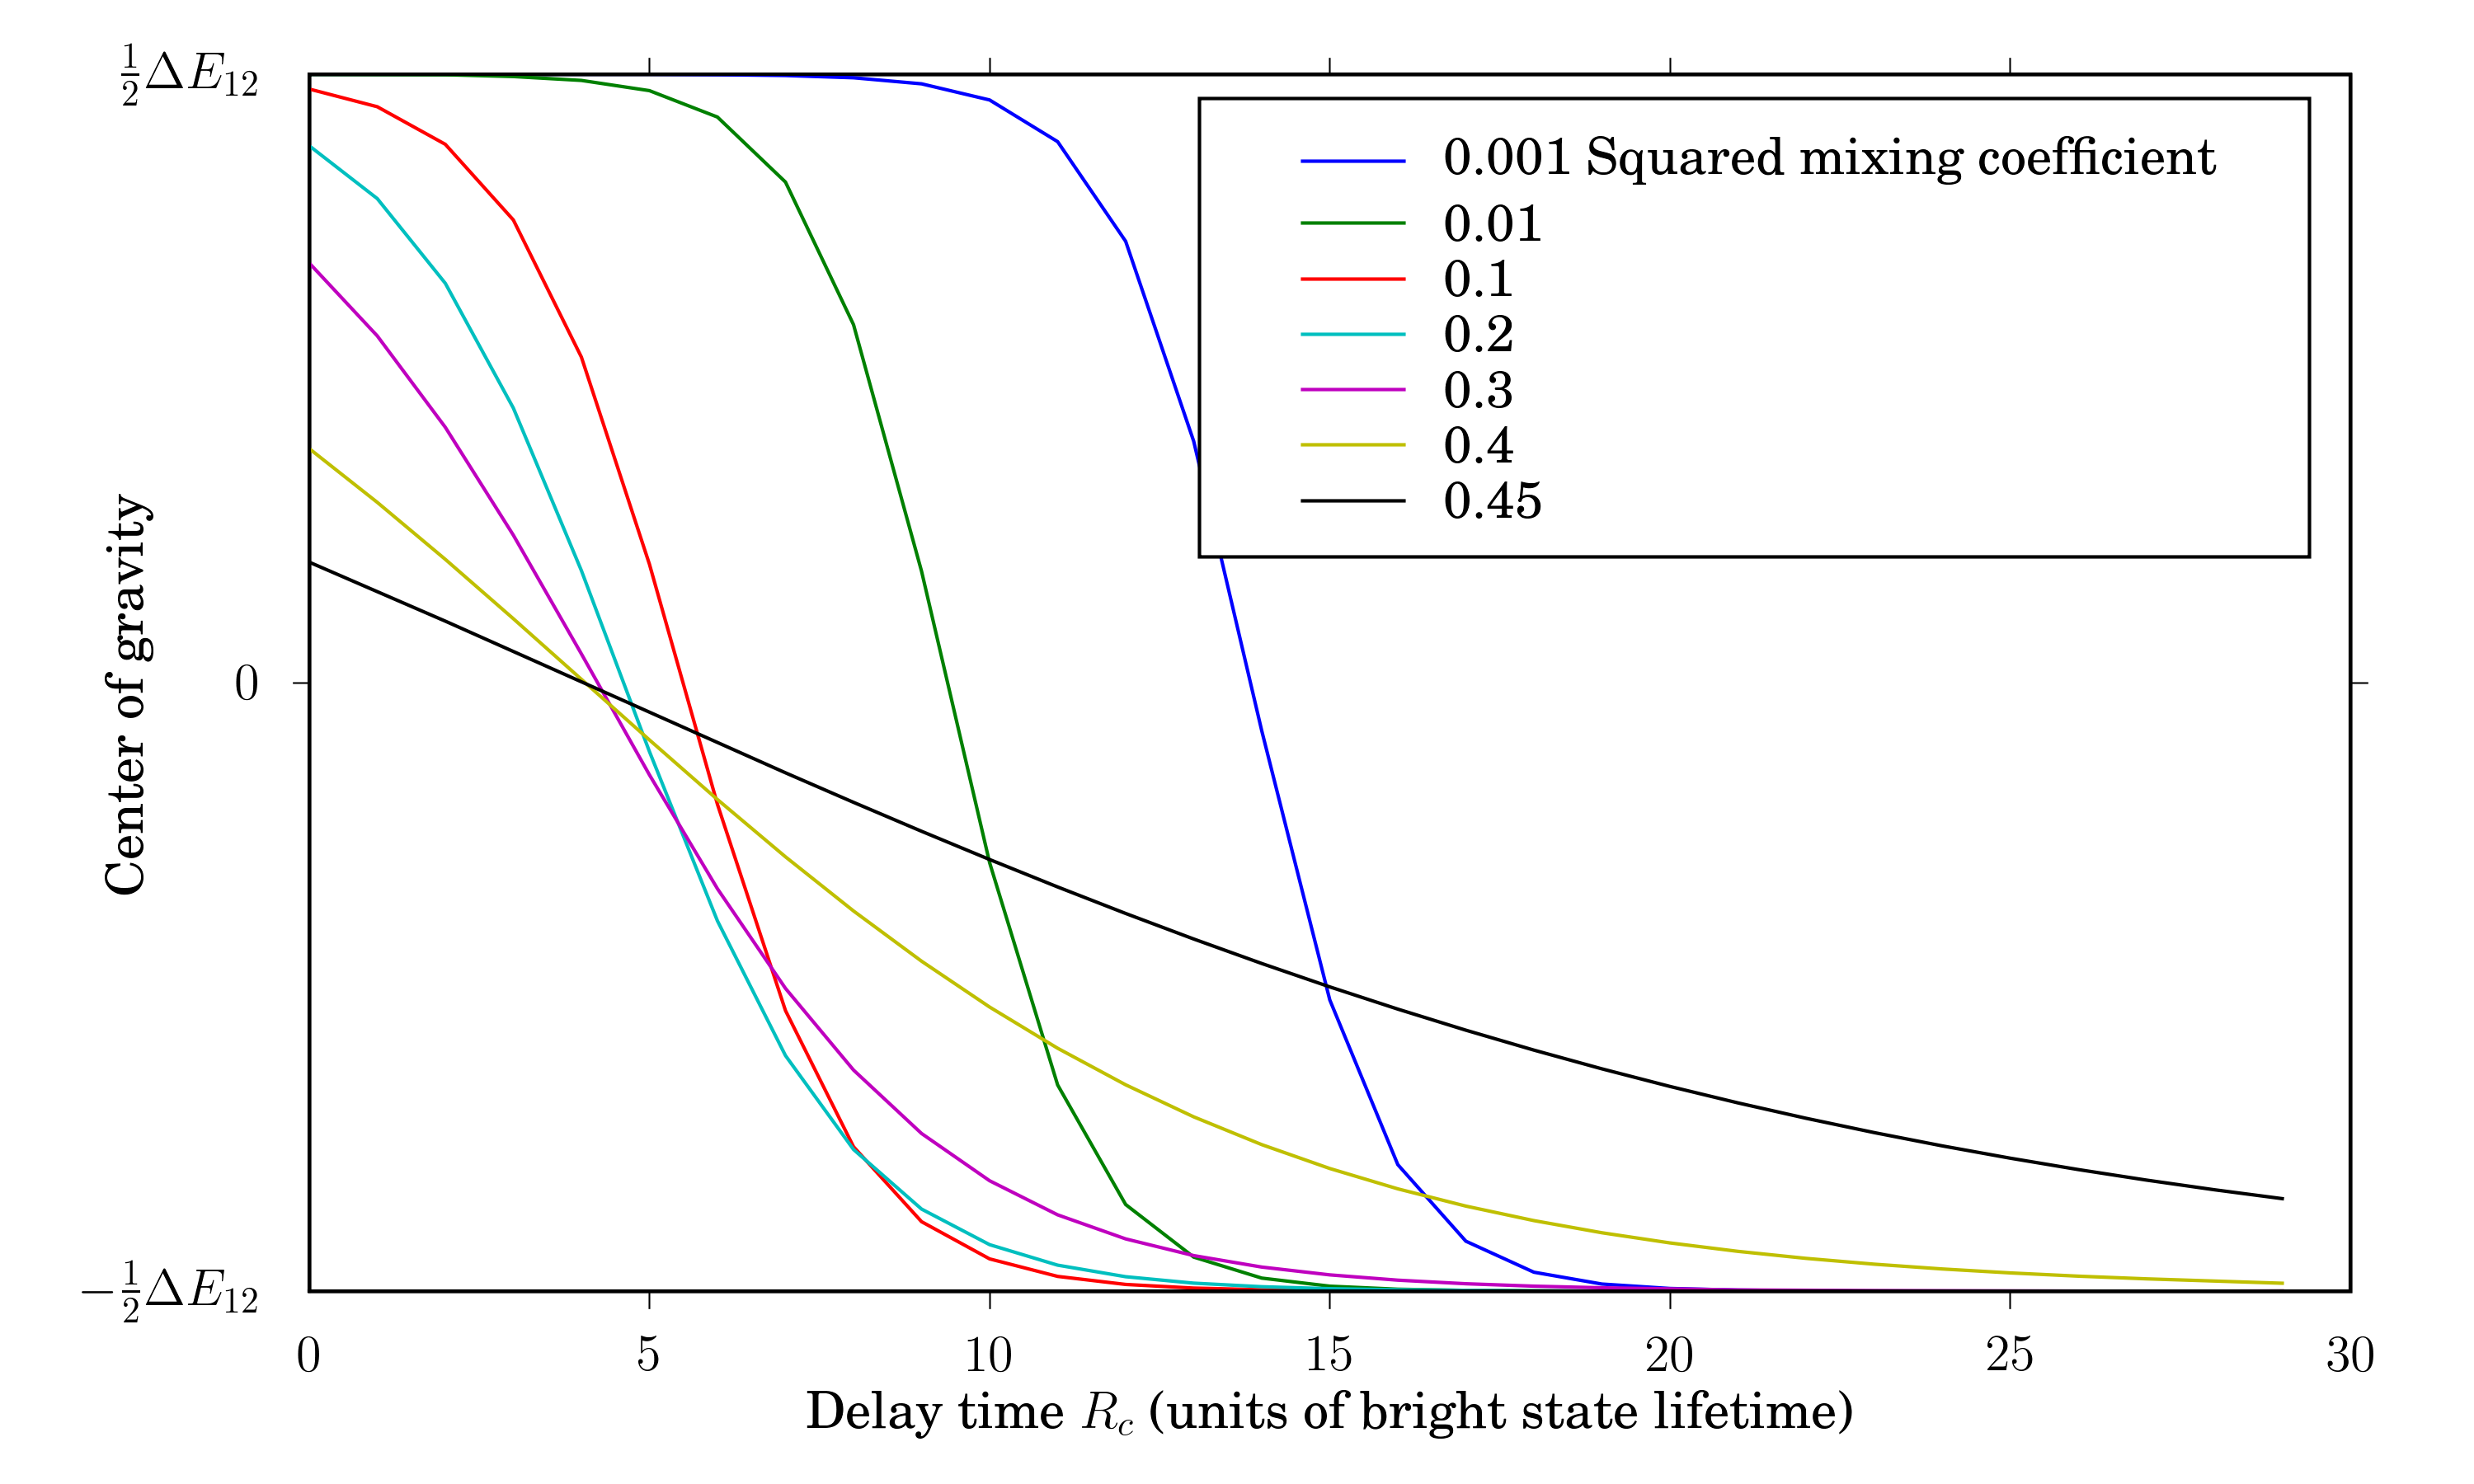
\includegraphics[width=6in]{cog-development.png}
\end{figure}

\subsection{Delayed fluorescence of a series of rotational
  transitions}

Information about the relative energy of a mediating level can be
recovered by studying the statistical properties of delayed
fluorescence as a function of rotational quantum number.  For a
near-symmetric prolate top in Hund's case ($b$), the selection rules
for spin-orbit coupling are \cite{stevens73}
\begin{equation}
  \begin{split}
    \Delta J &= 0 \\
    \Delta N &= 0, \pm 1\\
    \Delta K_a &= 0, \pm 1.
  \end{split}
\end{equation}

We take as a model system a series of equally spaced bright state
transitions with increasing rotational quantum number $J$.  The total
bright$\sim$dark coupling strength for each transition is function of
the energy separation between the bright state $\ket{s;J}$ and three
components of the non-local mediating level: $F_1$, $\ket{\ell;J-1}$;
$F_2$, $\ket{\ell;J}$; and $F_3$, $\ket{\ell;J+1}$.

\begin{figure}
  \caption{ Reduced term value plot of the three singlet$\sim$triplet
    roational components permitted by the spin-orbit operator in
    Hund's case ($b$).  The $F_1$ component corresponds to  }
  \label{fig:components}
  \centering
  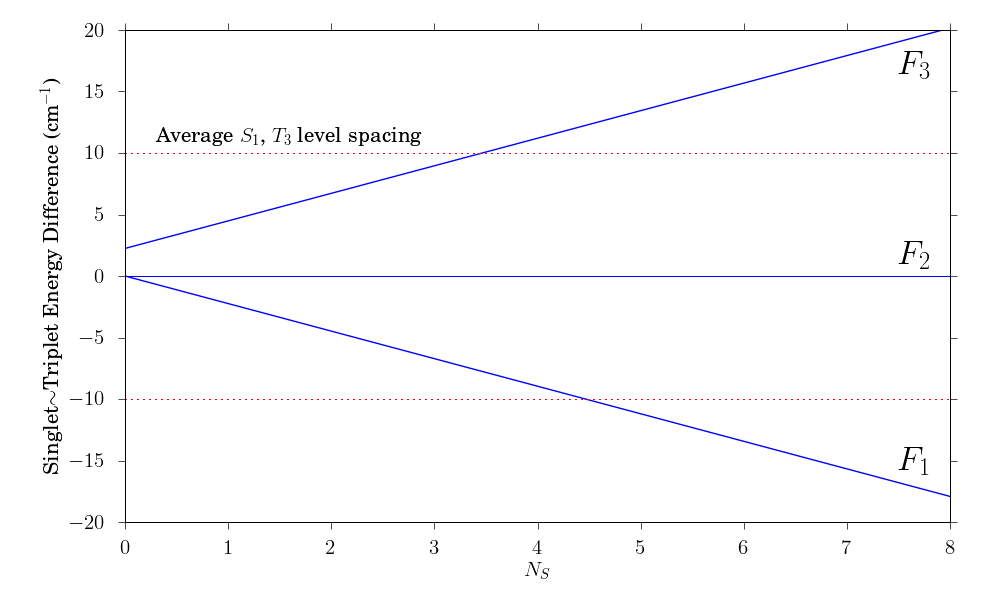
\includegraphics[width=6in]{f-components.png}
\end{figure}

To a very good approximation the total first-order spin-orbit matrix
element between two rovibrational states is given by the product of
three factors: an electronic spin-orbit matrix element, a vibrational
overlap factor, and a rotational factor arising from angular momentum
coupling rules.  The rotational factors are given for the general case
of polyatomic molecules by Stevens and Brand \cite{stevens73}.  

\POINT{Present rotational factors for first-order spin-orbit
  coupling.}  Plots of the spin-orbit rotational factors are presented
for singlet levels having $K$=0 (Figure
\ref{fig:rotational-factors-0}), $K$=1 (Figure
\ref{fig:rotational-factors-1}), and $K$=2 (Figure
\ref{fig:rotational-factors-2}).  With the exception of the $\Delta N
= \Delta K = 0$ components, the rotational factors quickly approach
their asymptotic ratios.  Even at low values of $J$, their variation
is less than a factor of 2 in all cases.  \POINT{These variations are
  trumped by energy denominator effects.}

\begin{figure}
  \caption{}
  \label{fig:rotational-factors-0}
  \centering
  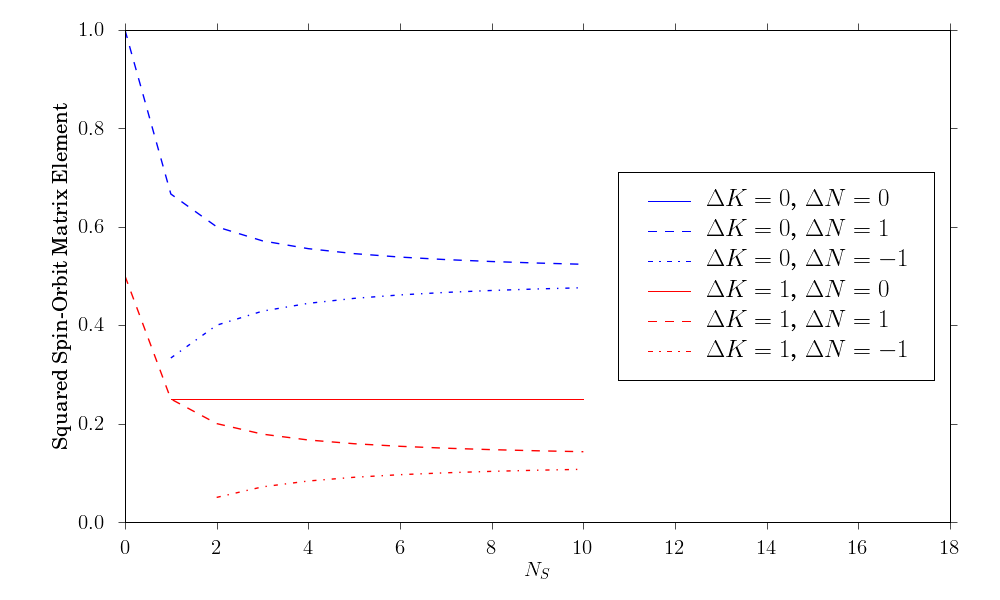
\includegraphics[width=6in]{rotational_factors_k0.png}
\end{figure}

\begin{figure}
  \caption{}
  \label{fig:rotational-factors-1}
  \centering
  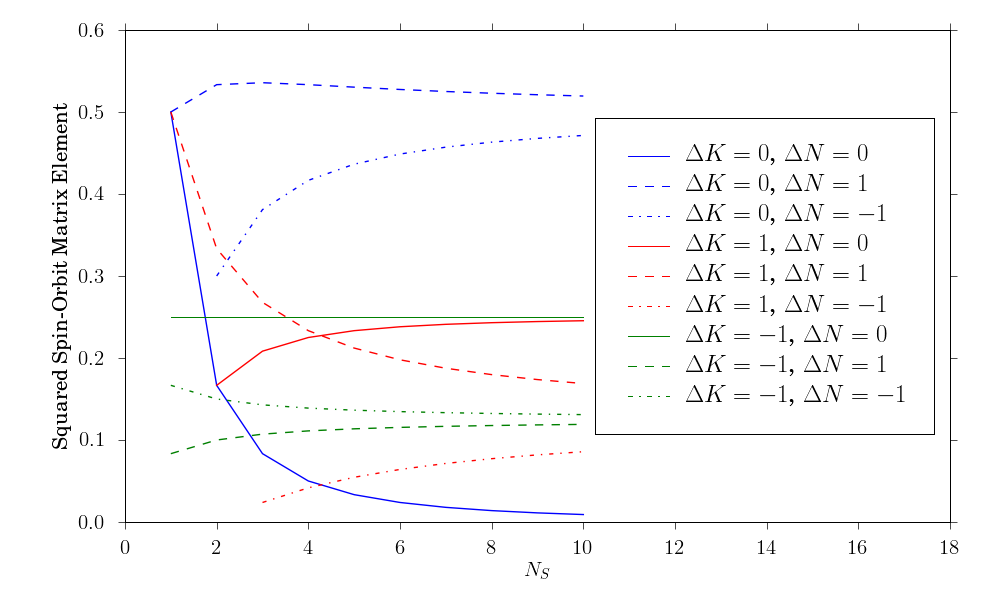
\includegraphics[width=6in]{rotational_factors_k1.png}
\end{figure}

\begin{figure}
  \caption{}
  \label{fig:rotational-factors-2}
  \centering
  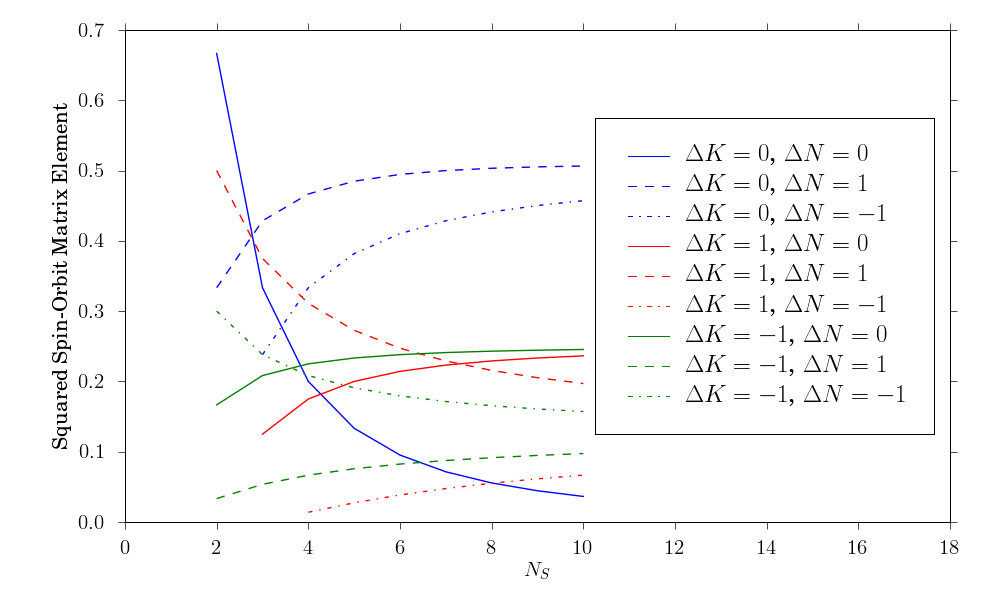
\includegraphics[width=6in]{rotational_factors_k2.png}
\end{figure}

The rotational dependence of energy differences for the three
components is
\begin{equation}
  \label{eq:components}
  \Delta E_{s\ell}(J) = 
  \begin{cases}
    \Delta B_{s\ell}J(J+1) + 2B_{\ell}J           
    & F_1 \text{ component}\\
    \Delta B_{s\ell}J(J+1)                      
    & F_2 \text{ component}\\
    \Delta B_{s\ell}J(J+1) - 2B_{\ell}J - 2B_{\ell} 
    & F_3 \text{ component}.\\
  \end{cases}
\end{equation}
\POINT{Give a general idea of the expected $T_3$ rotational constant
  from calculations and the RA experiment.  The product $\Delta
  B_{s\ell}J(J+1)$ is expected to remain small compared to $2BJ$.}

The effects of widely varying vibrational overlap factors will divide
$S_1 \sim T_3$ perturbations into two classes: those where
$H_{st}/\Delta E_{st} \ll 2B$, and those where $H_{st} / \Delta
E_{st}$ is on the order of $2B$.  Perturbations in the first class
will appear only once in the spectrum.  However, once a triplet level
with small vibrational overlap is found at a particular $J$, its
energy above or below the perturbed singlet level may be found
according to Equation \ref{eq:components}.

Perturbations falling into the second class will affect the
singlet$\sim$triplet coupling at several values of $J$; these are the
distant $T_3$ doorways with which we are most concerned.

% We simplify the above formulas by considering the \emph{average}
% energy difference, taking all components into account.  Giving equal
% weights to all components, the average energy separation is
% \begin{equation}
%   \Delta E_{s\ell}(J)_{\text{ave}} = \Delta B_{s\ell}J(J+1) - \frac{2}{3}B_{\ell}.
% \end{equation}
% We define a mixing coefficient $\alpha_{s\ell}$ between the bright
% state and the three components of the mediating level.  The mixing
% coefficient can be related to $\Delta E_{s\ell}$ using second order
% perturbation theory.  Introducing the average spin-orbit matrix
% element $H_{s\ell}$ for the three rotational components, the relation
% is $\alpha_{s\ell}(J) = H_{s\ell} / \Delta E_{s\ell}(J)$.  The
% relative strengths of the three components are given by simple
% formulas, which can be found in the literature.  We find that the
% functional dependence of the mixing coefficient between the bright
% state and the mediating components is
% \begin{equation}
%   \alpha_{s\ell}(J) = \frac{H_{s\ell}}{\Delta B_{s\ell}J(J+1)}.
% \end{equation}


\section{Experiment}

\TODO{Adapt this from paper.}  SEELEM is a versatile and sensitive
technique for investigating ``dark'' (weakly-fluorescing) metastable
molecules produced via laser excitation.1-6 In the SEELEM experiment,
a molecular beam of acetylene is excited by a $\sim$5 ns pulsed laser
into spin-rotation-vibration eigenstates of metastable electronic
states via weak, nominally forbidden transitions. After excitation,
the long-lived species must travel 35 cm before colliding with an Au
metal detector surface, where an electron is ejected in a
de-excitation process. Two criteria must be met for electron ejection
by a metastable species. First, the vertical electronic energy of the
metastable approaching the surface must exceed the work function of
the metal ($\Phi$Au = 5.1 eV). Second, the radiative lifetime of the
detected metastable eigenstate ($\tau_\text{rad}$) must exceed the
flight time from the point of laser excitation to the SEELEM surface
($\Delta$t=300 $\mu$s).

A sample of acetylene (BOC gases) at a backing pressure of one
atmosphere was pulsed through a 0.5 mm diameter nozzle operating at 10
Hz into a diffusion pumped vacuum chamber at $\sim$5x10-5 torr.  An Nd:YAG
pumped, frequency-doubled dye laser (220 nm) excited the acetylene
molecules in the pulsed jet expansion 2 cm downstream from the nozzle
orifice. UV-LIF was detected perpendicular to the plane defined by the
intersection of the pulsed molecular and laser beams using f/1.2
collection optics, a fluorescence filter (UG-11) to reduce scattered
laser light, and a PMT (Hamamatsu model R375). The fluorescence signal
was averaged by a boxcar integrator and recorded. For SEELEM
detection, the excited molecules in the pulsed expansion passed
through a conical skimmer (3mm diameter) to form a collimated
molecular beam, which traveled into a differentially pumped detector
chamber maintained at $\sim$4x10-7 torr, and collided with a heated (300
C) Au metal surface 35 cm downstream from the point of laser
excitation. The SEELEM detector was identical to that used in the
previously described apparatus with Au foil ($\Phi$ = 5.1 eV) as the
metal surface.  Particle counting techniques, including a multichannel
scalar (Oxford Tennelec Nucleus Inc. MCS-II v2.091) were used to
record laser-excited metastable counts as a function of laser
frequency, along with the simultaneously recorded LIF spectra. Both
SEELEM and LIF signals were averaged over 100 laser shots / data
point.

\section{Investigation of a near-isoenergetic set of $2^n3^m$ ($n+m=3$)
  vibrational levels}

\subsection{Observations}

\TODO{Figures of spectra for these bands (with assignments). See IGOR
  task list.}

\POINT{SEELEM spectrum of $2^2 3^1$ (Oct/Nov 2006, see ``similitude''
  calculations, p.62 of Sep 2006--Jan 2007 notebook.)}  This spectrum
is shown in Figure \ref{fig:spectrum-2231}.  For this band, several
scans were repeated with finer frequency steps.  Figure
\ref{fig:spectrum-2231-q123} shows the first three transitions of the
Q-branch.  Figure \ref{fig:spectrum-2231-q1r0} shows the two
transitions Q(1) and R(0).  The upper states for the transitions are
assigned as $J'=1$, and have $f$- and $e$-symmetry, respectively.
% Selection rules: Q   -> e-f
%                  P,R -> e-e, f-f

\begin{figure}
  \caption{
    % Simultaneously recorded LIF and SEELEM spectra of the
    % acetylene $V^2_04^2_0K^1_0$ $\tilde{A}^1A_u \leftarrow
    % \tilde{X}^1\Sigma_g$ transition.
    Simultaneously recorded surface electron ejection by laser excited
    metastables (SEELEM, upper trace) and ultraviolet laser-induced
    fluorescence (UV-LIF, lower trace) spectra of the $2^23^1$ $K_a$=1
    sublevel of the $\tilde{A}^1A_u \leftarrow \tilde{X} ^1\Sigma_g^+$
    electronic transition. A delayed, integrated fluorescence signal
    is shown as a dotted trace in the UV-LIF spectrum.}
  \label{fig:spectrum-2231}
  \centering
  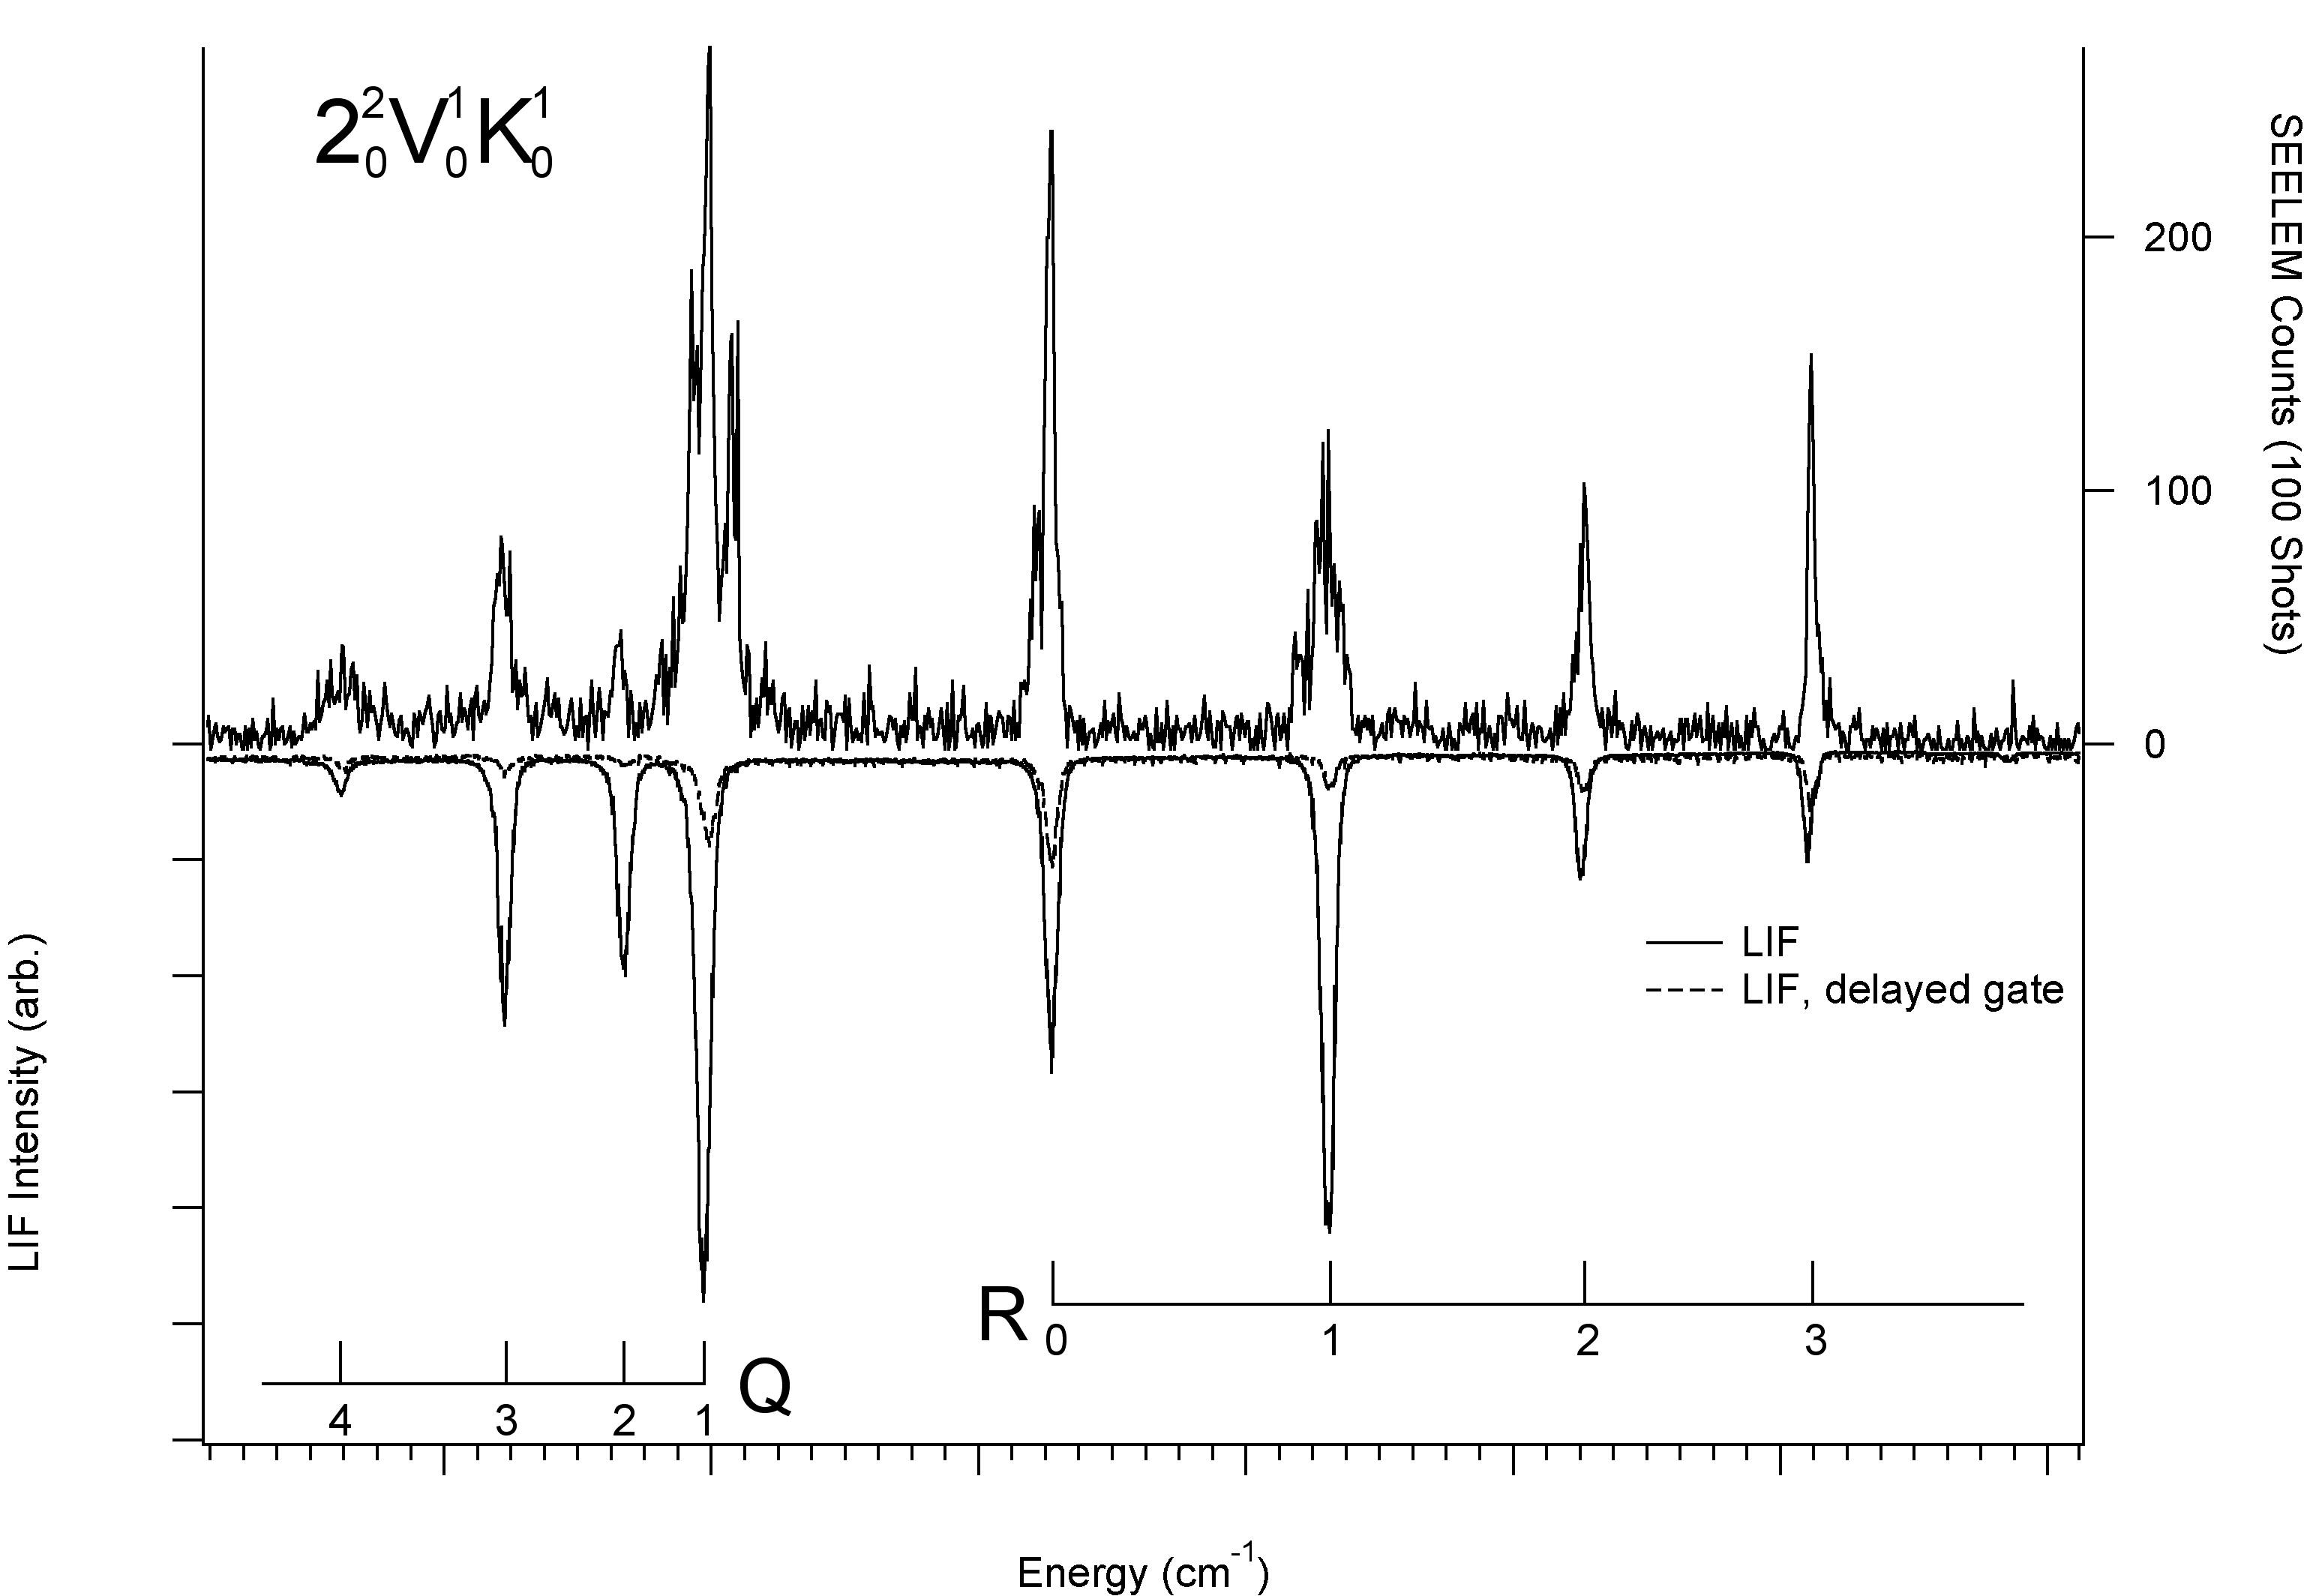
\includegraphics[width=8in,angle=90]{spectrum-2231.png}
\end{figure}

\begin{figure}
  \caption{
    % Simultaneously recorded LIF and SEELEM spectra of the
    % acetylene $V^2_04^2_0K^1_0$ $\tilde{A}^1A_u \leftarrow
    % \tilde{X}^1\Sigma_g$ transition.
    Simultaneously recorded surface electron ejection by laser excited
    metastables (SEELEM, upper trace) and ultraviolet laser-induced
    fluorescence (UV-LIF, lower trace) spectra of the $2^23^1$ $K_a$=1
    sublevel of the $\tilde{A}^1A_u \leftarrow \tilde{X} ^1\Sigma_g^+$
    electronic transition. A delayed, integrated fluorescence signal
    is shown as a dotted trace in the UV-LIF spectrum.}
  \label{fig:spectrum-2231-q123}
  \centering
  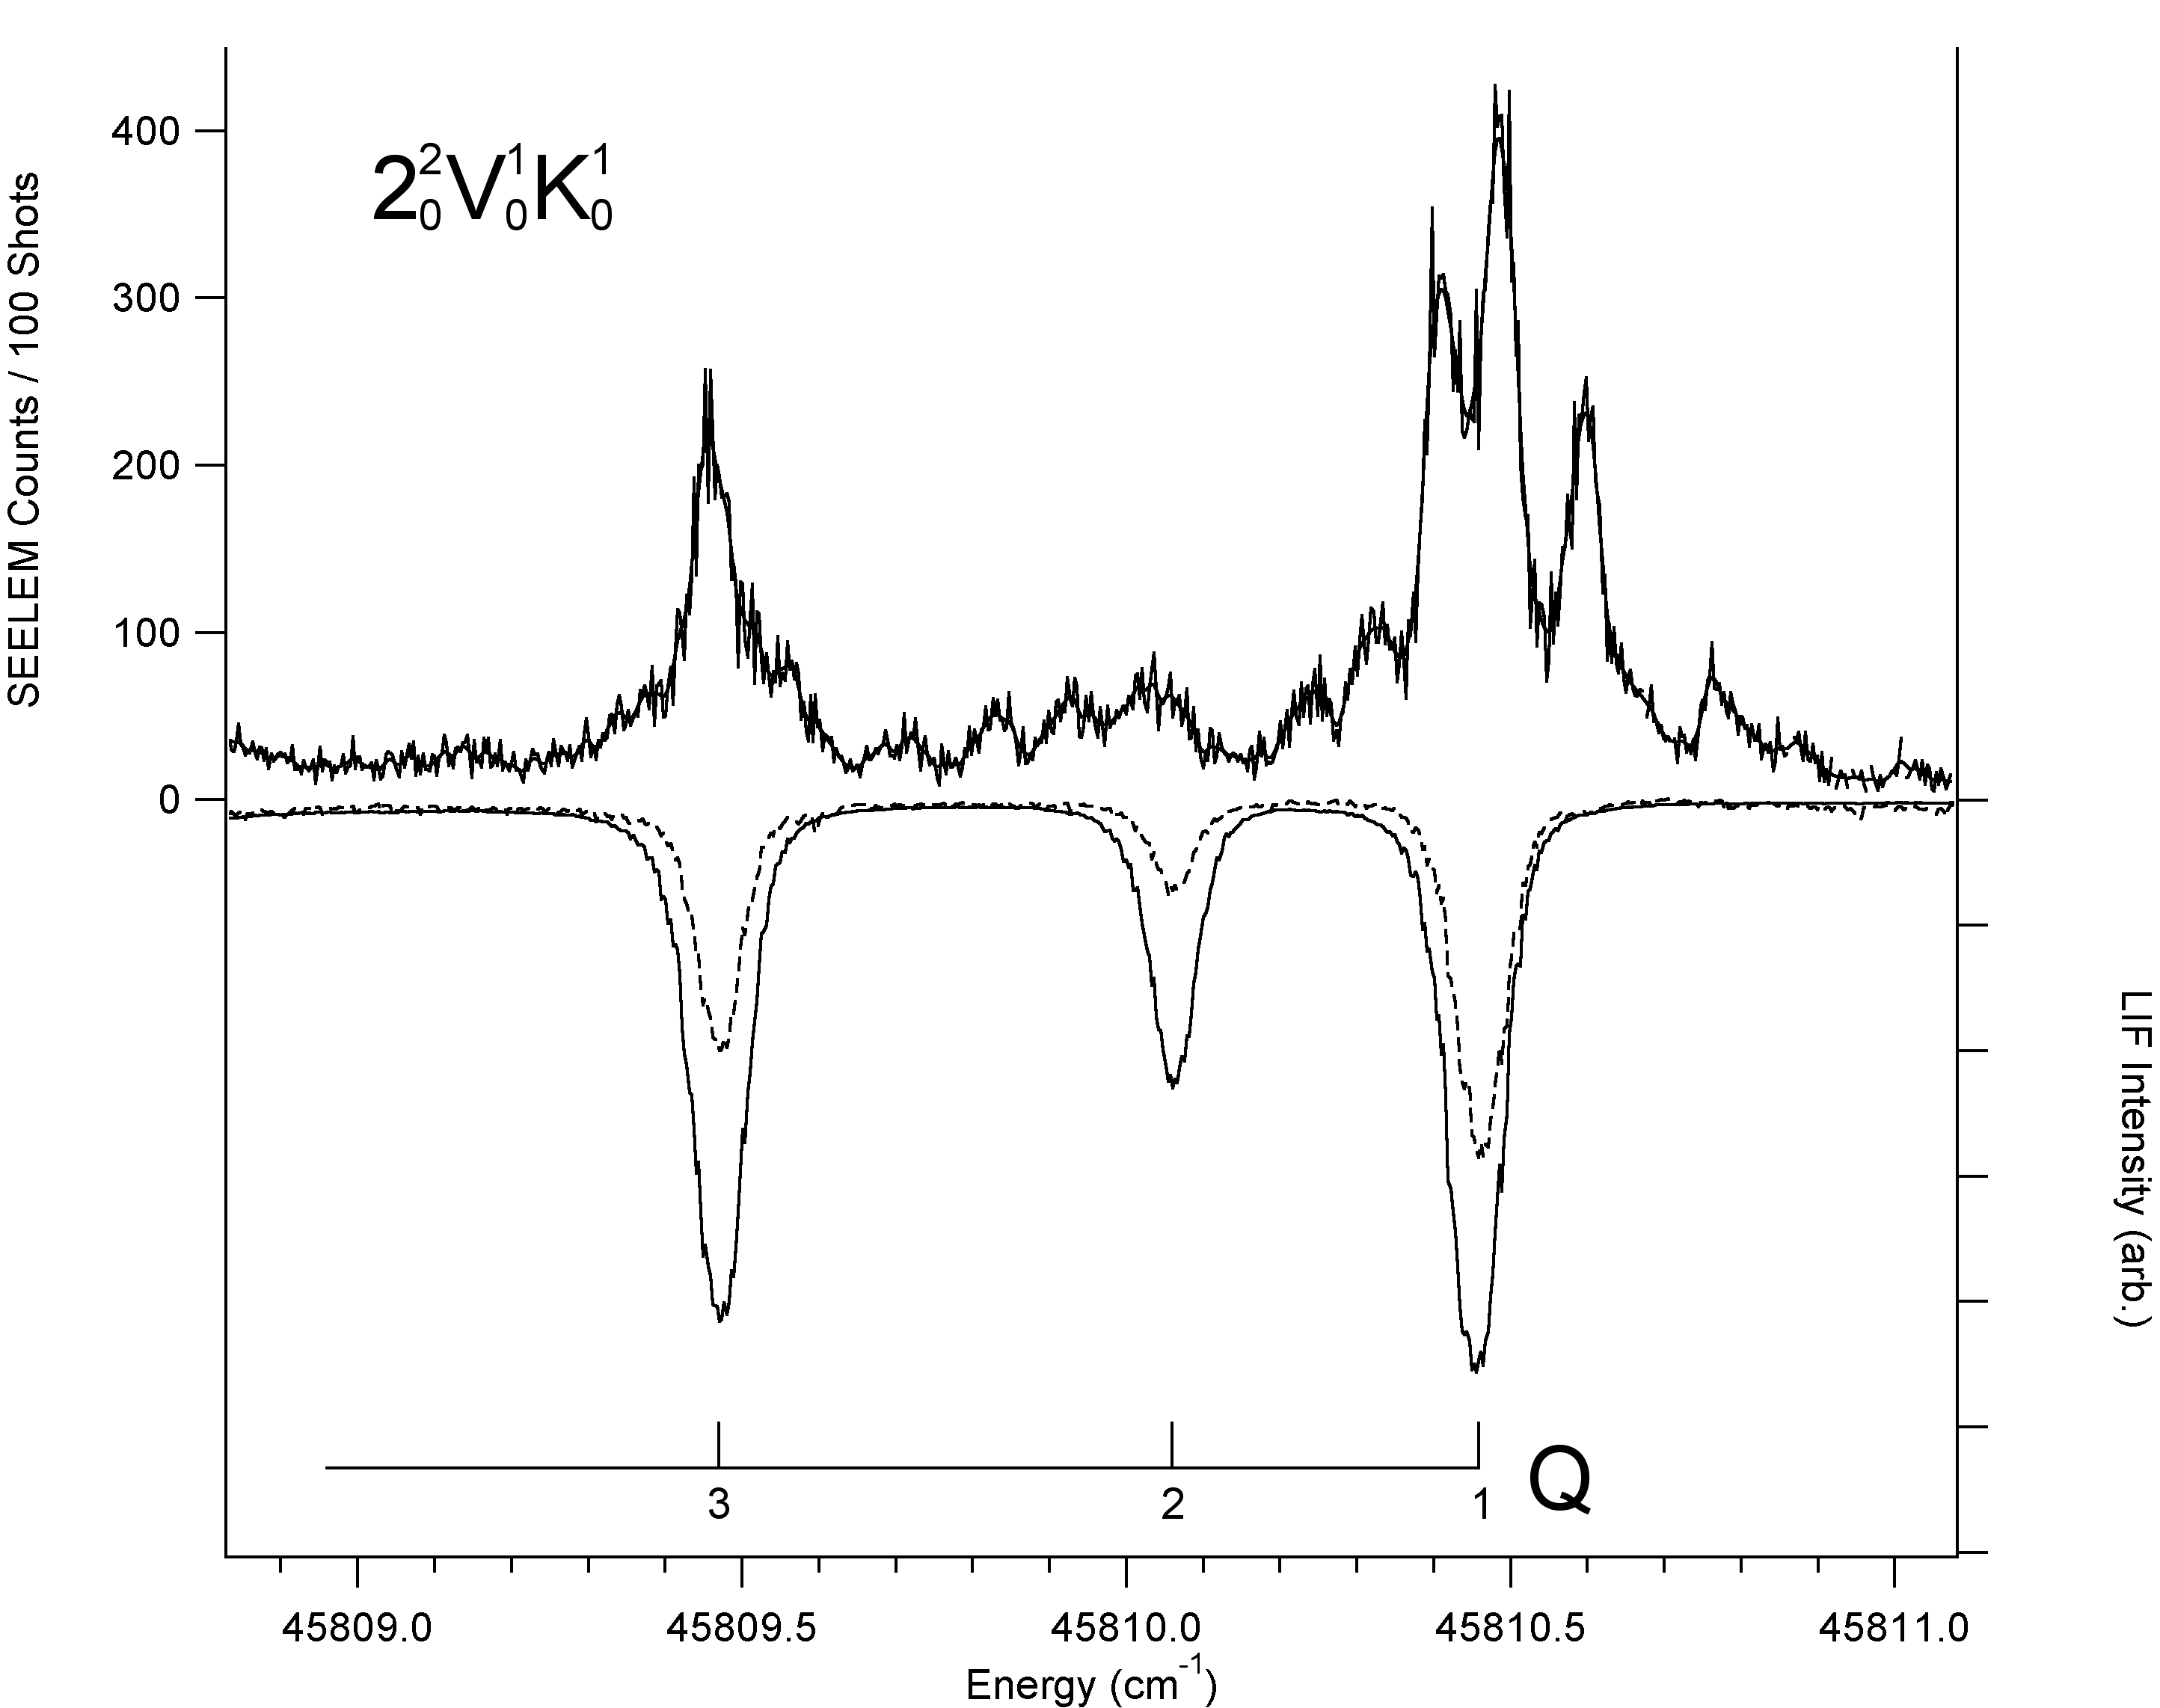
\includegraphics[width=6in]{spectrum-2231-Q123.png}
\end{figure}

\begin{figure}
  \caption{
    % Simultaneously recorded LIF and SEELEM spectra of the
    % acetylene $V^2_04^2_0K^1_0$ $\tilde{A}^1A_u \leftarrow
    % \tilde{X}^1\Sigma_g$ transition.
    Simultaneously recorded surface electron ejection by laser excited
    metastables (SEELEM, upper trace) and ultraviolet laser-induced
    fluorescence (UV-LIF, lower trace) spectra of the $2^23^1$ $K_a$=1
    sublevel of the $\tilde{A}^1A_u \leftarrow \tilde{X} ^1\Sigma_g^+$
    electronic transition. A delayed, integrated fluorescence signal
    is shown as a dotted trace in the UV-LIF spectrum.}
  \label{fig:spectrum-2231-q1r0}
  \centering
  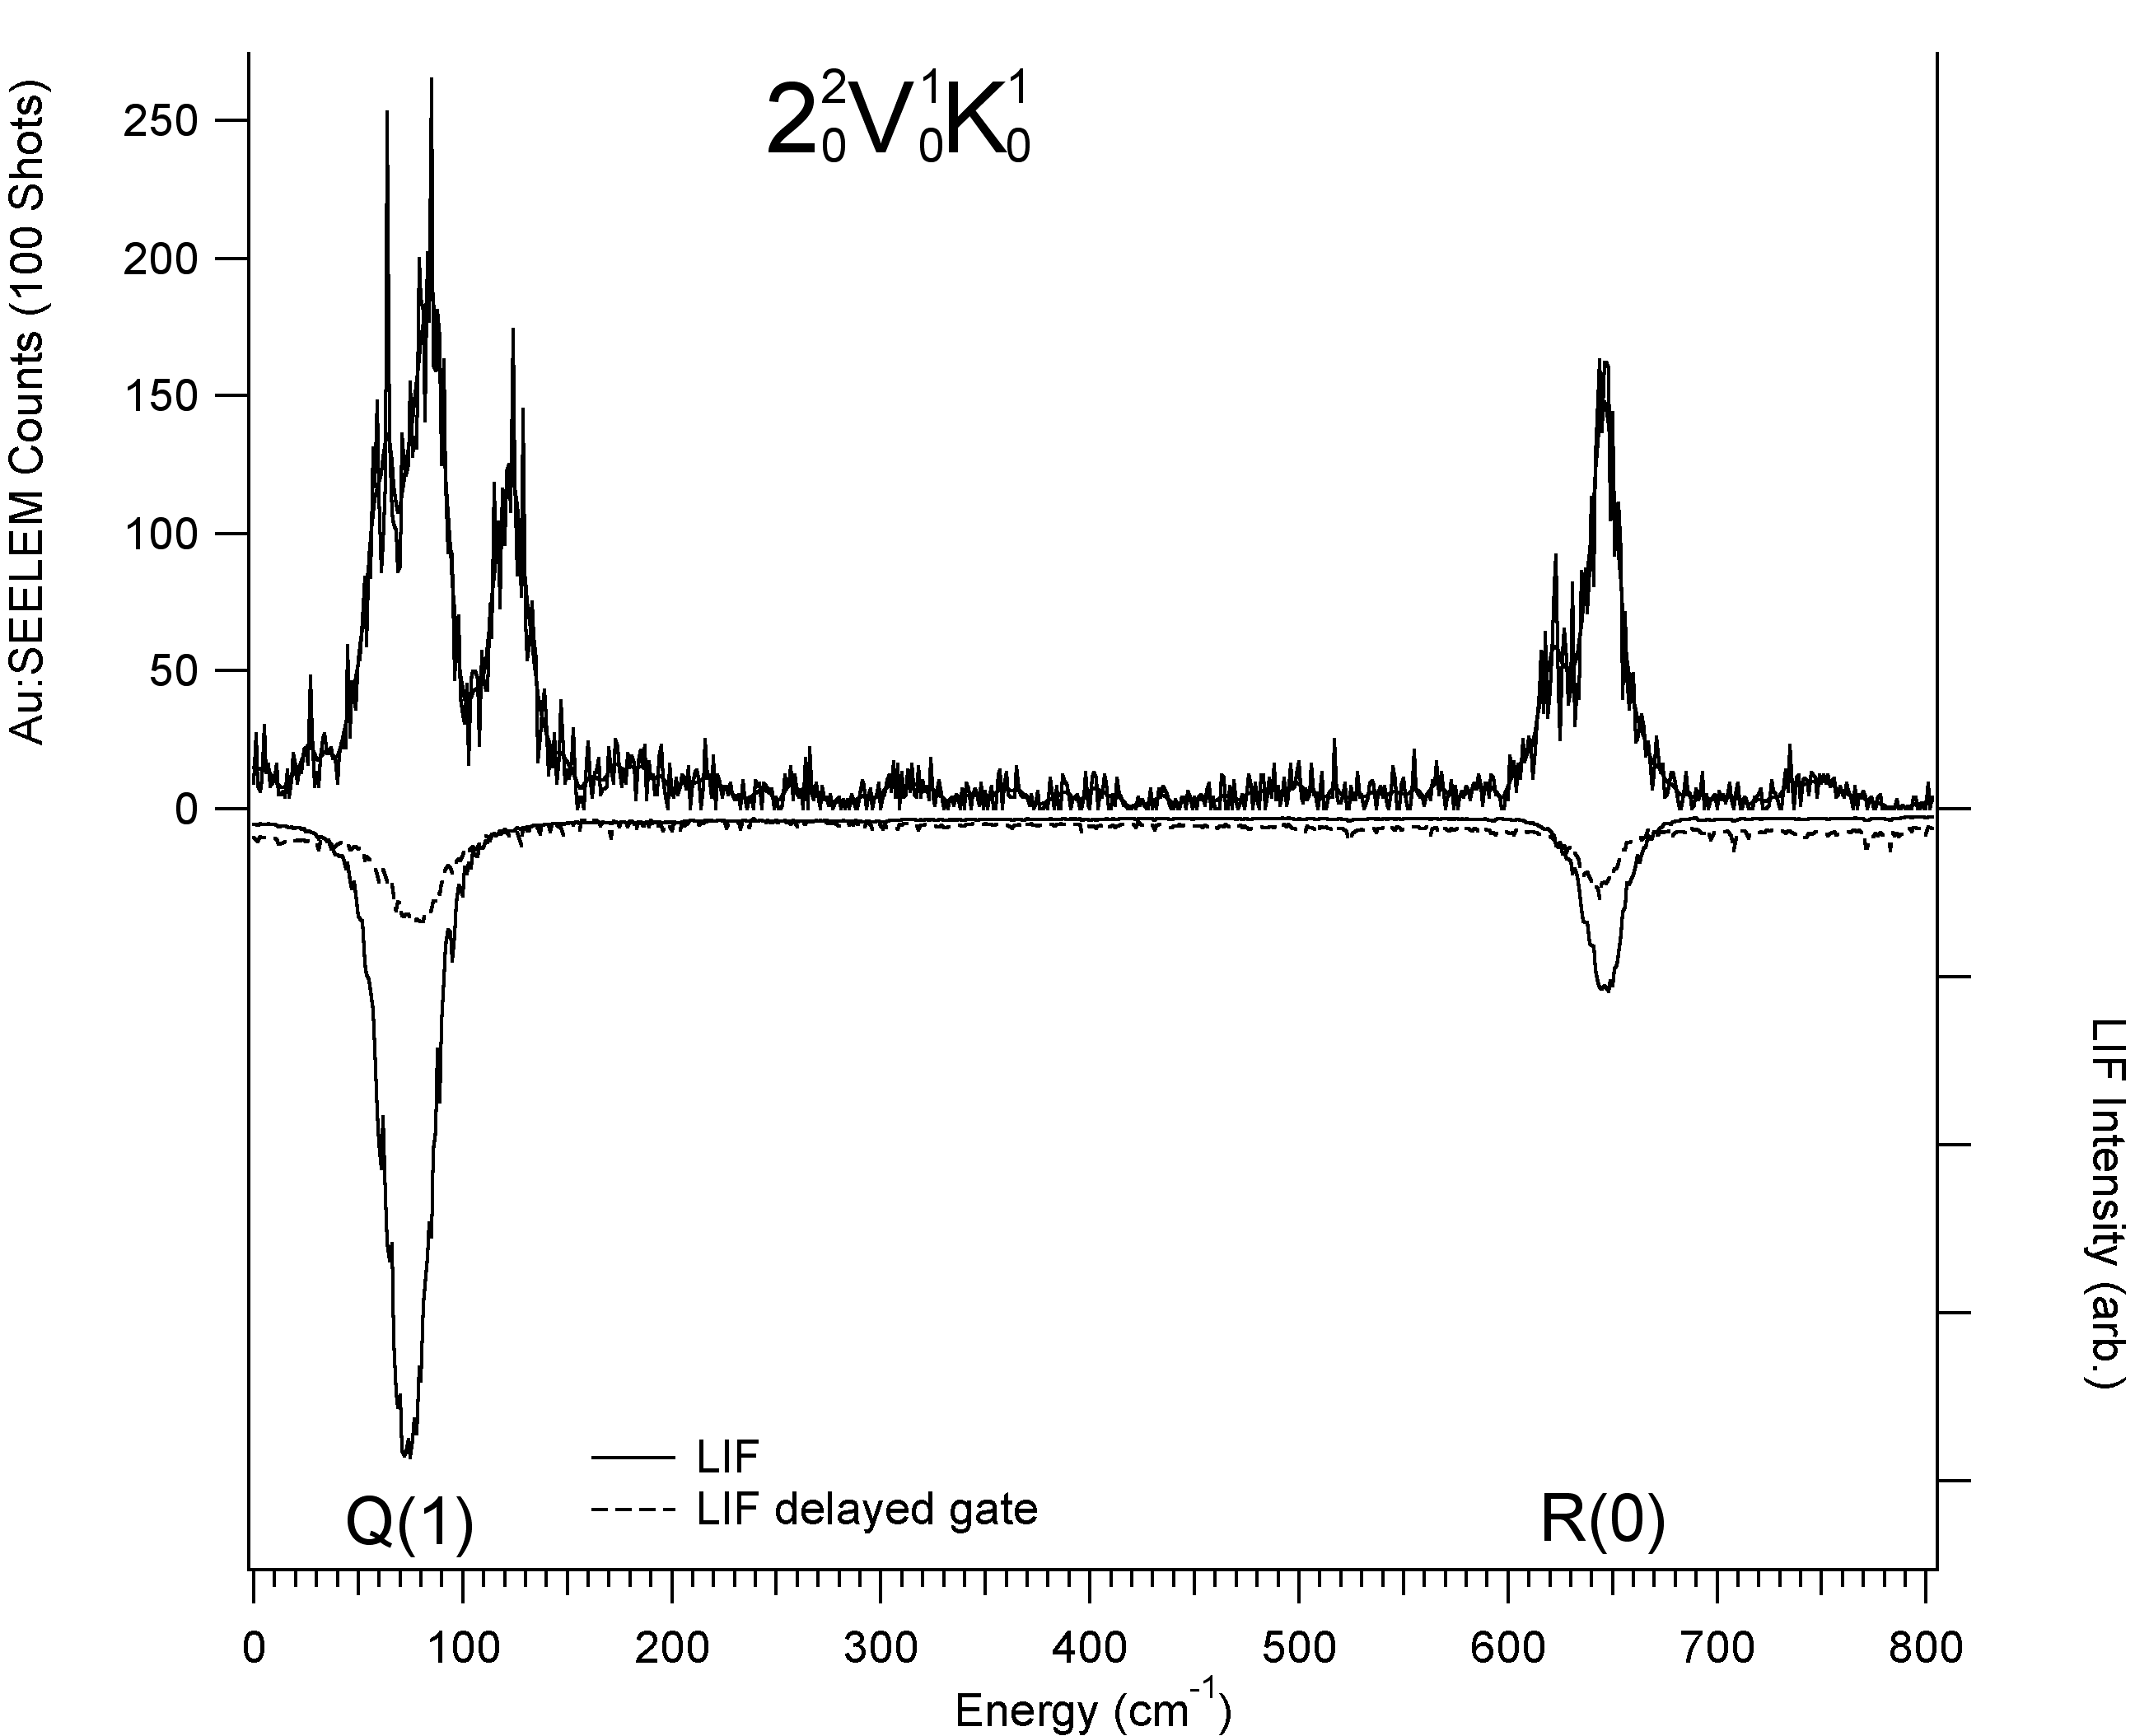
\includegraphics[width=6in]{spectrum-2231-Q1R0.png}
\end{figure}

\POINT{SEELEM spectrum of $2^1 3^2$ P, Q-branch (See Jan 16A+B,
  p.124--127 of 9/2006--1/2007 notebook, also assignments on p.2 of
  1/2007--3/2007 notebook.)}  This spectrum is shown in Figure
\ref{fig:spectrum-2132}.

\begin{figure}
  \caption{
    % Simultaneously recorded LIF and SEELEM spectra of the
    % acetylene $V^2_04^2_0K^1_0$ $\tilde{A}^1A_u \leftarrow
    % \tilde{X}^1\Sigma_g$ transition.
    Simultaneously recorded surface electron ejection by laser excited
    metastables (SEELEM, upper trace) and ultraviolet laser-induced
    fluorescence (UV-LIF, lower trace) spectra of the $2^13^2$ $K_a$=1
    sublevel of the $\tilde{A}^1A_u \leftarrow \tilde{X} ^1\Sigma_g^+$
    electronic transition. A delayed, integrated fluorescence signal
    is shown as a dotted trace in the UV-LIF spectrum.}
  \label{fig:spectrum-2132}
  \centering
  \includegraphics[width=8in,angle=90]{spectrum-2132.pdf}
\end{figure}


\POINT{SEELEM spectrum of $3^3$ $K=2$ hot band (See Jan 22C, p.31,34
  of 1/2007--3/2007 notebook.)}  This spectrum is shown in Figure
\ref{fig:spectrum-33k2}.

\begin{figure}
  \caption{
    Simultaneously recorded surface electron ejection by laser excited
    metastables (SEELEM, upper trace) and ultraviolet laser-induced
    fluorescence (UV-LIF, lower trace) spectra of the $3^3$ $K_a$=2
    sublevel of the $\tilde{A}^1A_u \leftarrow \tilde{X} ^1\Sigma_g^+$
    electronic transition. A delayed, integrated fluorescence signal
    is shown as a dotted trace in the UV-LIF spectrum.}
  \label{fig:spectrum-33k2}
  \centering
  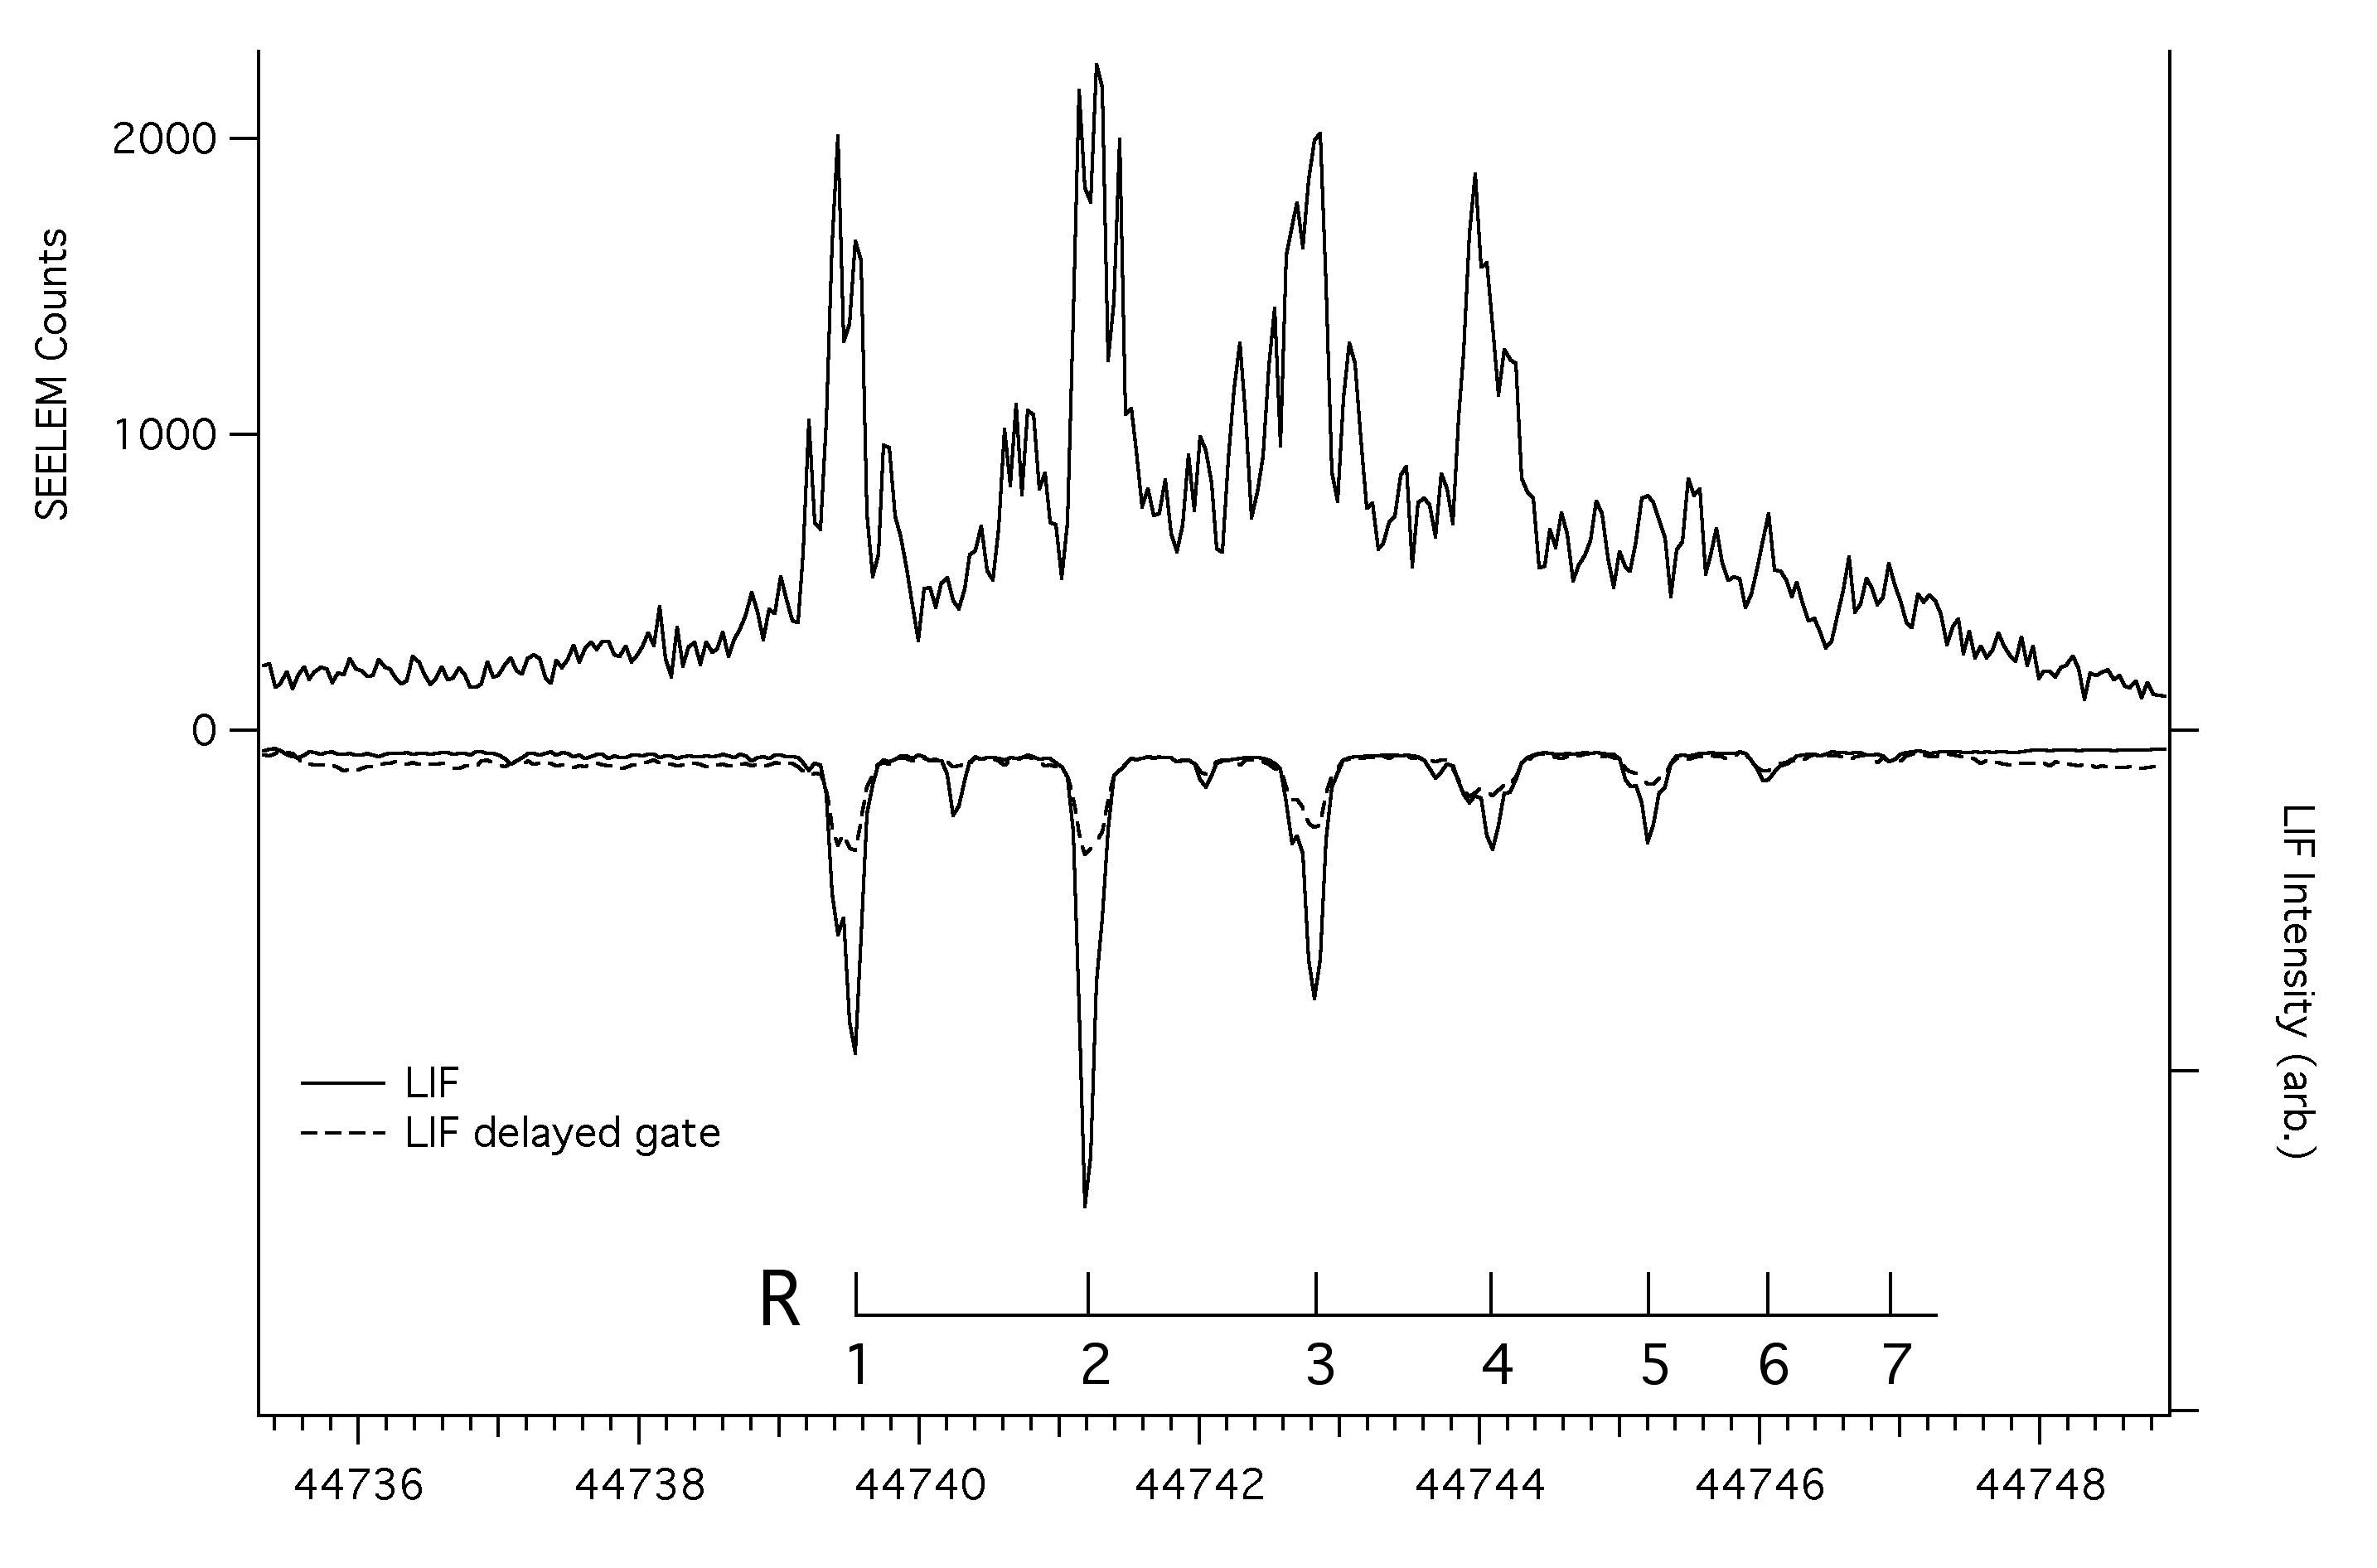
\includegraphics[width=8in,angle=90]{spectrum-33k2.png}
\end{figure}

\POINT{SEELEM spectrum of $3^2 4^2$ with lone SEELEM peak in band gap
  (December 2006, p.86 of 9/2006--1/2007 notebook.)}  This spectrum is
shown in Figure \ref{fig:spectrum-32b2}.

\begin{figure}
  \caption{
    % Simultaneously recorded LIF and SEELEM spectra of the
    % acetylene $V^2_04^2_0K^1_0$ $\tilde{A}^1A_u \leftarrow
    % \tilde{X}^1\Sigma_g$ transition.
    Simultaneously recorded surface electron ejection by laser excited
    metastables (SEELEM, upper trace) and ultraviolet laser-induced
    fluorescence (UV-LIF, lower trace) spectra of the $3^24^2$ $K_a$=1
    sublevel of the $\tilde{A}^1A_u \leftarrow \tilde{X} ^1\Sigma_g^+$
    electronic transition. A delayed, integrated fluorescence signal
    is shown as a dotted trace in the UV-LIF spectrum.}
  \label{fig:spectrum-32b2}
  \centering
  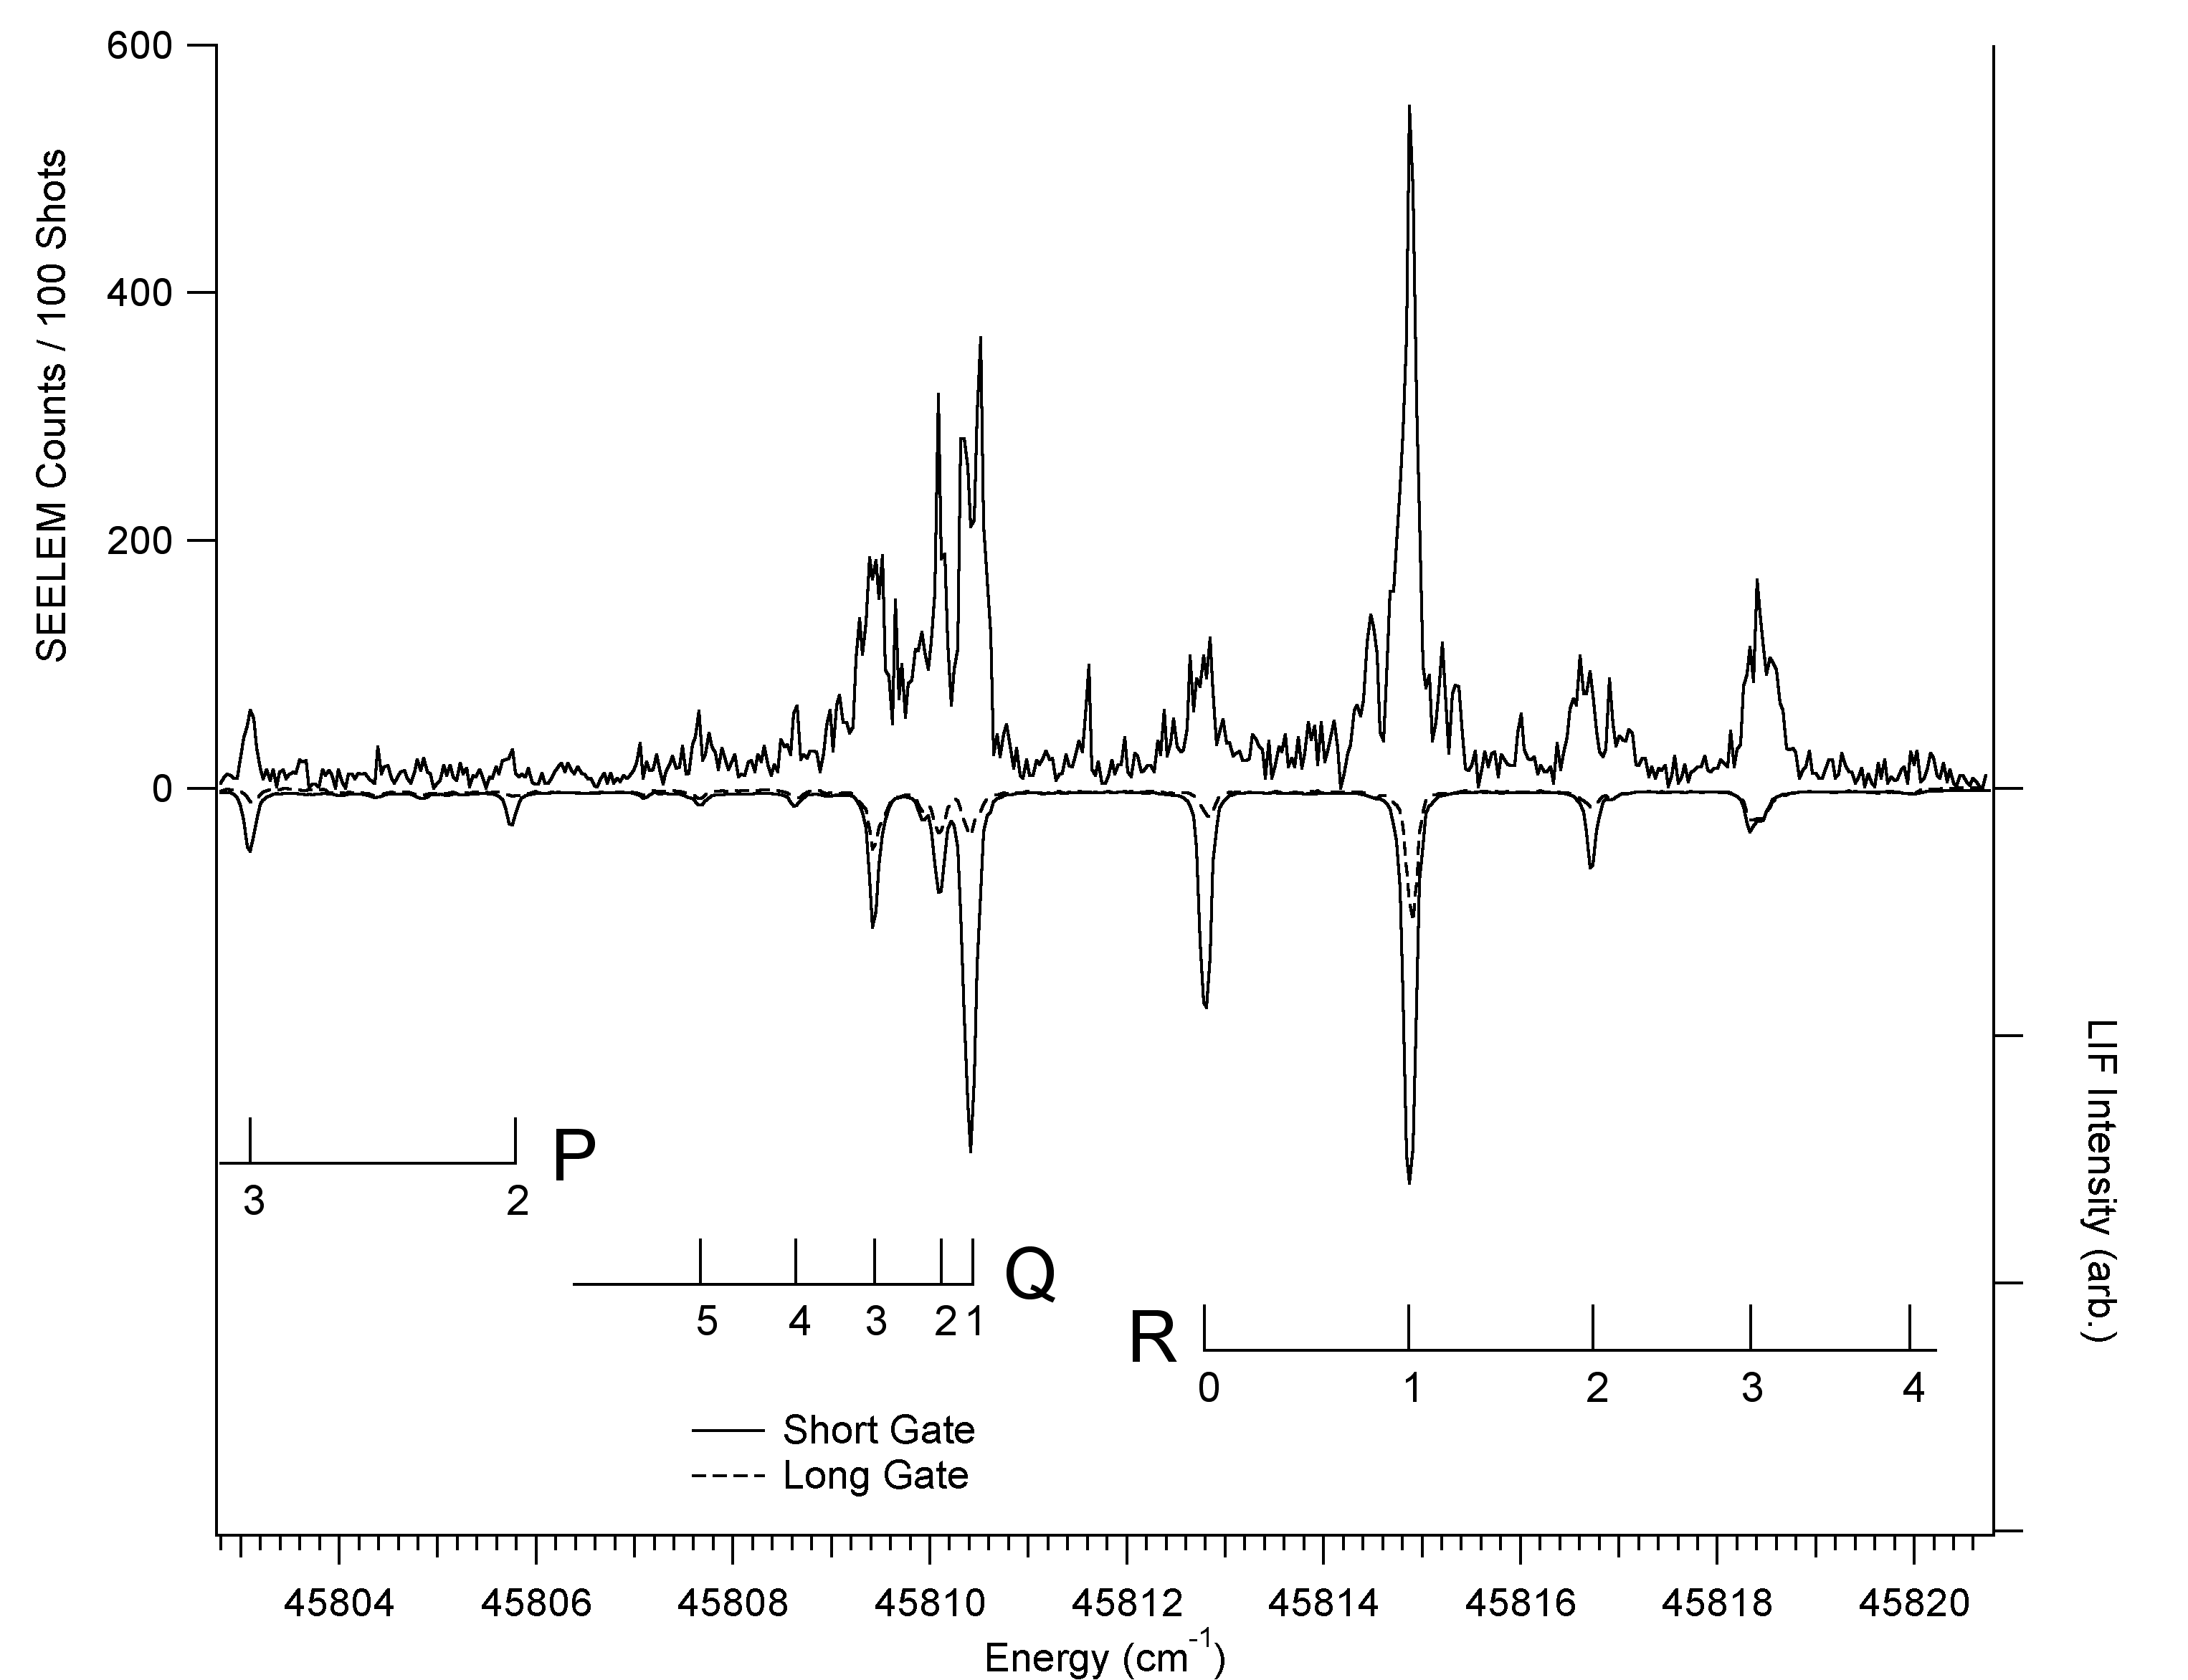
\includegraphics[width=7.5in,angle=90]{spectrum-32b2.png}
\end{figure}

\subsection{LIF/SEELEM intensity distributions}

\subsection{Analysis}

\POINT{Analyze the remaining bands under the assumption of distant
  doorway coupling via $T_3$.  Include center-of-gravity metrics,
  lifetime/gated fluorescence metrics, and intensity distributions.}

\section{Conclusion}

\POINT{The LIF/SEELEM spectra for the progression of $2^n3^m$ levels
  shows the expected trends for strong coupling.}

\POINT{Prospects for other vibrational levels: (1) levels with
  perturbations observed by the singlets, (2) other $3^2B^2$ polyad
  members, (3) other K-sublevels in the FC active modes.}


\bibliography{master}
\bibliographystyle{plain}
\end{document}